%%%%%%%%%%%%%%%%%%%%%%%%%%%%%%%%%%%%
% Slide options
%%%%%%%%%%%%%%%%%%%%%%%%%%%%%%%%%%%%

% Option 1: Slides with solutions

\documentclass[slidestop,compress,mathserif]{beamer}
\newcommand{\soln}[1]{\textit{#1}}
\newcommand{\solnGr}[1]{#1}

% Option 2: Handouts without solutions

%\documentclass[11pt,containsverbatim,handout]{beamer}
%\usepackage{pgfpages}
%\pgfpagesuselayout{4 on 1}[letterpaper,landscape,border shrink=5mm]
%\newcommand{\soln}[1]{ }
%\newcommand{\solnGr}{ }


%%%%%%%%%%%%%%%%%%%%%%%%%%%%%%%%%%%%
% Style
%%%%%%%%%%%%%%%%%%%%%%%%%%%%%%%%%%%%

\usetheme{metropolis}

%%%%%%%%%%%%%%%%
% Packages
%%%%
%%%%%% pacotes para acentos
%\usepackage[english]{babel}
%\usepackage[latin1]{inputenc}
\usepackage[utf8]{inputenc} 
\usepackage[brazil]{babel}
\usepackage[T1]{fontenc}

\usepackage{geometry}
\usepackage{graphicx}
\usepackage{amssymb}
%\usepackage{cancel}
\usepackage{epstopdf}
\usepackage{amsmath}  	% this permits text in eqnarray among other benefits
\usepackage{url}		% produces hyperlinks
\usepackage{hyperref}	% allows for color usage in tables

\usepackage{colortbl}	% allows for color usage in tables
\usepackage{multirow}	% allows for rows that span multiple rows in tables
\usepackage{color}		% this package has a variety of color options
\usepackage{pgf}
\usepackage{calc}
\usepackage{ulem}
\usepackage{multicol}
\usepackage{textcomp}
\usepackage{txfonts}
\usepackage{listings}
\usepackage{tikz}
\usepackage{array}
\usepackage{wasysym}
\usepackage{fancyvrb}
\usepackage{ragged2e} % justifica o texto
\usepackage{scalefnt} %redimensiona o tamanho da tabela comando = \scalefont{0.5}

%%%%%%%%%%%%%%%%
% Remove navigation symbols
%%%%%%%%%%%%%%%%

\setbeamertemplate{navigation symbols}{}

%%%%%%%%%%%%%%%%
% User defined colors
%%%%%%%%%%%%%%%%

\xdefinecolor{oiB}{rgb}{0.22,0.52,0.72}
\definecolor{oiG}{rgb}{.298,.447,.114}
\xdefinecolor{hlblue}{rgb}{0.051,0.65,1}
\xdefinecolor{gray}{rgb}{0.5, 0.5, 0.5}
\xdefinecolor{darkGray}{rgb}{0.3, 0.3, 0.3}
\xdefinecolor{darkerGray}{rgb}{0.2, 0.2, 0.2}
\xdefinecolor{rubineRed}{rgb}{0.89,0,0.30}
\xdefinecolor{irishGreen}{rgb}{0,0.60,0}	
\definecolor{lightGreen}{rgb}{0.387,0.581,0.148} 

%%%%%%%%%%%%%%%%
% Template colors
%%%%%%%%%%%%%%%%

%\setbeamercolor*{palette primary}{fg=white,bg= oiB!80!black!90}
%\setbeamercolor*{palette secondary}{fg=black,bg= oiB!80!black}
%\setbeamercolor*{palette tertiary}{fg=white,bg= oiB!80!black!80}
%\setbeamercolor*{palette quaternary}{fg=white,bg= oiB}
%\setbeamercolor{structure}{fg= oiB}
%\setbeamercolor{frametitle}{bg= oiB!90}
%\setbeamertemplate{blocks}[shadow=false]
%\setbeamersize{text margin left=2em,text margin right=2em}

%\setbeamercolor{code body}{bg=gray!20!white!80,fg=black}


%%%%%%%%%%%%%%%%
% Get rid of fancy enumerated list bullets
%%%%%%%%%%%%%%%%

%\setbeamertemplate{enumerate items}[default]

%%%%%%%%%%%%%%%%
% Custom commands
%%%%%%%%%%%%%%%%

% degree
\newcommand{\degree}{\ensuremath{^\circ}}

% cite
\newcommand{\ct}[1]{
\vfill
{\tiny #1}}

% Note
\newcommand{\Note}[1]{
\rule{2.5cm}{0.25pt} \\ \textit{\footnotesize{\textcolor{rubineRed}{Note:} \textcolor{darkerGray}{#1}}}}

% Remember
\newcommand{\Remember}[1]{\textit{\scriptsize{\textcolor{orange}{Remember:} #1}}}

% expected counts
\newcommand{\ex}[1]{\textit{\textcolor{blue}{#1}}}

% red
\newcommand{\red}[1]{\textit{\textcolor{rubineRed}{#1}}}

% pink
\newcommand{\pink}[1]{\textit{\textcolor{rubineRed!90!white!50}{#1}}}

% green
\newcommand{\green}[1]{\textit{\textcolor{irishGreen}{#1}}}

% orange
\newcommand{\orange}[1]{\textit{\textcolor{orange}{#1}}}

% links: webURL, webLin, appLink
\newcommand{\webURL}[1]{\urlstyle{same}{ \textit{\textcolor{darkGray}{\url{#1}}}}}
\newcommand{\webLink}[2]{\href{#1}{\textcolor{darkGray}{{#2}}}}
\newcommand{\appLink}[2]{\href{#1}{\textcolor{white}{{#2}}}}

% mail
\newcommand{\mail}[1]{\href{mailto:#1}{\textit{\textcolor{darkGray}{#1}}}}

% highlighting: hl, hlGr, mathhl
\newcommand{\hl}[1]{\textit{\textcolor{hlblue}{#1}}}
\newcommand{\hlGr}[1]{\textit{\textcolor{lightGreen}{#1}}}
\newcommand{\mathhl}[1]{\textcolor{hlblue}{\ensuremath{#1}}}

% two col: two columns
\newenvironment{twocol}[4]{
\begin{columns}[c]
\column{#1\textwidth}
#3
\column{#2\textwidth}
#4
\end{columns}
}

% slot (for probability calculations)
\newenvironment{slot}[2]{
\begin{array}{c} 
\underline{#1} \\ 
#2
\end{array}
}

% pr: left and right parentheses
\newcommand{\pr}[1]{
\left( #1 \right)
}

% solnMult: solutions for practice questions

\newcommand{\solnMult}[1]{
\item[] \vspace{-0.59cm}
\only<1>{\item #1}
\soln{\only<2->{\item \orange{#1}}}
}

% cancel
\newcommand{\cancel}[1]{%
    \tikz[baseline=(tocancel.base)]{
        \node[inner sep=0pt,outer sep=0pt] (tocancel) {#1};
        \draw[red, line width=0.5mm] (tocancel.south west) -- (tocancel.north east);
    }%
}

% removepagenumbers
\newcommand{\removepagenumbers}{% 
  \setbeamertemplate{footline}{}
}

%%%%%%%%%%%%%%%%
% Custom boxes
%%%%%%%%%%%%%%%%

% app: application exercise

\setbeamercolor{app body}{fg=oiG}

\newcommand{\app}[1]{
\begin{beamerboxesrounded}[shadow = false, lower = app body]{}
#1
\end{beamerboxesrounded}
}

% dq: discussion question

\setbeamercolor{disc ques body}{fg=oiB}

\newcommand{\dq}[1]{
\begin{beamerboxesrounded}[shadow = false, lower = disc ques body]{}
#1
\end{beamerboxesrounded}
}

% pq: practice question

\setbeamercolor{prac ques body}{fg=oiB}

\newcommand{\pq}[1]{
\begin{beamerboxesrounded}[shadow = false, lower = prac ques body]{}
#1
\end{beamerboxesrounded}
}

% formula

\setbeamercolor{formula body}{fg=oiB!55!black!95}

\newcommand{\formula}[1]{
\begin{beamerboxesrounded}[shadow = false, lower = formula body]{}
#1
\end{beamerboxesrounded}
}


%%%%%%%%%%%%%%%%
% Change margin
%%%%%%%%%%%%%%%%

\newenvironment{changemargin}[2]{%
\begin{list}{}{%
\setlength{\topsep}{0pt}%
\setlength{\leftmargin}{#1}%
\setlength{\rightmargin}{#2}%
\setlength{\listparindent}{\parindent}%
\setlength{\itemindent}{\parindent}%
\setlength{\parsep}{\parskip}%
}%
\item}{\end{list}}

%%%%%%%%%%%%%%%%
% Footnote
%%%%%%%%%%%%%%%%

\long\def\symbolfootnote[#1]#2{\begingroup%
\def\thefootnote{\fnsymbol{footnote}}\footnote[#1]{#2}\endgroup}

%%%%%%%%%%%%%%%%
% Commands from the book
%%%%%%%%%%%%%%%%

\newenvironment{data}[1]{\texttt{#1}}{}
\newenvironment{var}[1]{\texttt{#1}}{}
\newenvironment{resp}[1]{\texttt{#1}}{}

%%%%%%%%%%%%%%%%
% Graphics
%%%%%%%%%%%%%%%%

\DeclareGraphicsRule{.tif}{png}{.png}{`convert #1 `dirname #1`/`basename #1 .tif`.png}


%%%%%%%%%%%%%%%%%%%%%%%%%%%%%%%%%%%%
% Preamble
%%%%%%%%%%%%%%%%%%%%%%%%%%%%%%%%%%%%

\title[Chp 4: Foundations for inference]{Capítulo 4: Fundamentos para inferência}
\institute{$\:$ \\ {\footnotesize Slides desenvolvidos por Mine \c{C}etinkaya-Rundel of OpenIntro. \\
Os slides podem ser copiados, editados e / ou compartilhados via \webLink{http://creativecommons.org/licenses/by-sa/3.0/us/}{CC BY-SA license.} \\
Algumas imagens podem ser incluídas em diretrizes de uso justo (propósitos educacionais).}}
\date{}


%%%%%%%%%%%%%%%%%%%%%%%%%%%%%%%%%%%%
% Begin document
%%%%%%%%%%%%%%%%%%%%%%%%%%%%%%%%%%%%

\begin{document}


%%%%%%%%%%%%%%%%%%%%%%%%%%%%%%%%%%%%
% Title page
%%%%%%%%%%%%%%%%%%%%%%%%%%%%%%%%%%%%

{
\addtocounter{framenumber}{-1} 
{\removepagenumbers 
\usebackgroundtemplate{
\includegraphics[width=\paperwidth]{../OpenIntro_Grid_4_3-01.jpg}}

\begin{frame}


\includegraphics[width=10cm]{../logo_ead.png}

\small	{\textit{Tradução e adaptação: }\\
Priscilla Gnewuch, Márcia Helena Barbian e Maitê Mückler}

\footnotesize{Slides baseados no material desenvolvido por Mine \c{C}etinkaya-Rundel of OpenIntro. }

\footnotesize{Tanto este material  \href{https://github.com/Probabilidade-e-Estatistica-EAD/slides_openintro}{adaptado}, quanto o \href{https://github.com/OpenIntroStat/openintro-statistics-slides}{original}, podem ser copiados, editados e/ou compartilhados. O material adaptado está licenciado sob a Licença Creative Commons Atribuição  4.0 Internacional. Para ver uma cópia desta licença, visite \href{http://creativecommons.org/licenses/by/4.0/} {http://creativecommons.org/licenses/by/4.0/}}


\hfill 
\includegraphics[width=15mm]{../ufrgs-logo}
\includegraphics[width=20mm]{../logoime}
\includegraphics[width=20mm]{../sead-logo}


\end{frame}

\begin{frame}

\titlepage

\end{frame}
}
}


%%%%%%%%%%%%%%%%%%%%%%%%%%%%%%%%%%%%
% Sections
%%%%%%%%%%%%%%%%%%%%%%%%%%%%%%%%%%%%

%%%%%%%%%%%%%%%%%%%%%%%%%%%%%%%%%%%%

\section{4.1. Estimativas pontuais e variabilidade de amostragem}

%%%%%%%%%%%%%%%%%%%%%%%%%%%%%%%%%%%%

\begin{frame}
\frametitle{Estimativas pontuais e erro}
\justifying

\begin{itemize}
    \justifying
    \footnotesize
    \item Frequentemente estamos interessados em \hl{parâmetros populacionais}.
    \item É difícil coletar todos os dados de uma população (fazer um censo). Por isso usamos \hl{estatísticas da amostra} como \hl{estimativas pontuais} dos parâmetros desconhecidos da população de interesse.
    \item \hl{Erro} na estimativa = diferença entre o parâmetro da população e a estatística da amostra.
    \item \hl{Viés} é uma tendência sistemática que super ou subestima o verdadeiro parâmetro da população.
    \item \hl{Erro de amostragem} descreve o quanto uma estimativa tende a variar de uma amostra para outra.
    \item Grande parte das estatísticas concentra-se em compreender e quantificar o erro de amostragem, e o \hl{tamanho da amostra} é útil para quantificar esse erro.
\end{itemize}

\end{frame}

\begin{frame}
\justifying
\dq{Suponha que nós amostramos aleatoriamente 1.000 adultos de cada estado nos EUA. Você esperaria que as médias amostrais de suas alturas sejam as mesmas, um pouco diferentes ou muito diferentes?}

\pause
\justifying
\soln{Esperamos que as médias amostrais não sejam as mesmas, mas apenas um pouco diferentes.}

\end{frame}


\begin{frame}
\frametitle{}

\begin{center}
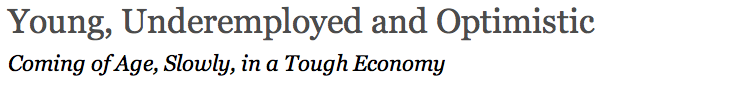
\includegraphics[width=0.95\textwidth]{4-1_var_in_est/pew1.png} \\
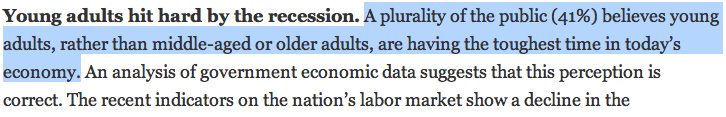
\includegraphics[width=0.95\textwidth]{4-1_var_in_est/pew2.png} \\
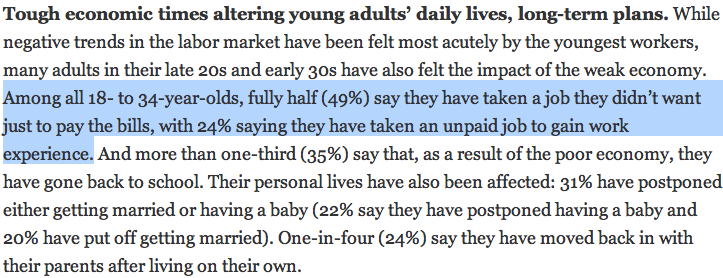
\includegraphics[width=0.95\textwidth]{4-1_var_in_est/pew3.png}
\end{center}

\ct{\webURL{http://pewresearch.org/pubs/2191/young-adults-workers-labor-market-pay-careers-advancement-recession}}

\end{frame}


%%%%%%%%%%%%%%%%%%%%%%%%%%%%%%%%%%%%

\begin{frame}
\frametitle{Tradução do texto: Young, Underemployed and Optmistic}
\justifying
\textbf{Jovem, Subempregado e Otimista}\\
\vspace{0.1 cm}

\justifying
\textit{Envelhecer, lentamente, em uma economia difícil}.\\
\vspace{0.4 cm}

\justifying
\footnotesize{
\textbf{Jovens adultos são duramente atingidos pela recessão}. \hl{Uma grande parte do público (41\%) acredita que os jovens adultos, ao invés dos adultos de meia-idade ou mais os velhos, estão tendo o momento mais difícil na economia atual}. Uma análise dos dados econômicos do governo sugere que essa percepção está correta. Os indicadores recentes sobre o mercado de trabalho da nação mostram um declínio na taxa de desemprego. No entanto, desde 2010, a proporção de jovens adultos de 18 a 24 anos atualmente empregados (54\%) é a menor desde que o governo começou a coletar esses dados em 1948. E a diferença no emprego entre os jovens e todos os adultos em idade ativa - 15 pontos percentuais - é o mais amplo da registrado na história. Além disso, os jovens adultos empregados em período integral tiveram uma queda maior nos seus ganhos semanais (menos 6\%) do que qualquer outro grupo etário nos últimos quatro anos.}\\

\end{frame}
%%%%%%%%%%%%%%%%%%%%%%%%%%%%%%%%%%%%

\begin{frame}
\frametitle{Tradução do texto: Young, Underemployed and Optmistic}

\justifying
\footnotesize{
\textbf{Tempos econômicos difíceis que alteram a vida cotidiana dos jovens adultos e seus planos de longo prazo}. Embora as tendências negativas no mercado de trabalho tenham sido mais fortemente sentidas pelos trabalhadores mais jovens, muitos adultos com cerca de 20 e 30 anos também sentiram o impacto da fraca economia. \hl{Entre todas as pessoas de 18 a 34 anos, metade (49\%) diz que aceitou um trabalho que não queria apenas para poder pagar as contas, com 24\% dizendo que aceitou um emprego não remunerado para ganhar experiência profissional}. E mais de um terço (35\%) dizem que, como resultado da economia pobre, voltaram à escola. Suas vidas pessoais também foram afetadas: 31\% adiaram o casamento ou a gravidez (22\% disseram que adiaram ter um bebê e 20\% adiaram o casamento). Um em quatro (24\%) dizem que voltaram a morar com os pais depois de viverem sozinhos.}

\end{frame}
%%%%%%%%%%%%%%%%%%%%%%%%%%%%%%%%%%%%

\begin{frame}
\frametitle{Margem de erro}

\begin{center}
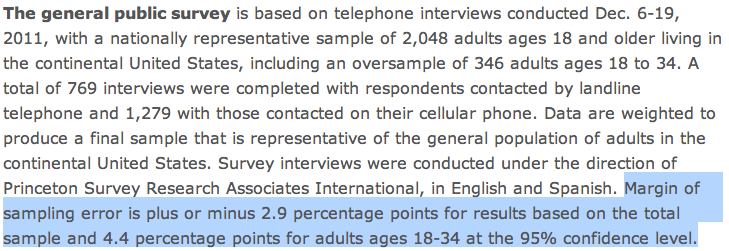
\includegraphics[width=0.95\textwidth]{4-1_var_in_est/pew4.png}
\end{center}

\end{frame}
%%%%%%%%%%%%%%%%%%%%%%%%%%%%%%%%%%%%

\begin{frame}
\frametitle{Tradução do texto: Margem de Erro}
\justifying
\small{
\textbf{A pesquisa do público geral} é baseada em entrevistas telefônicas realizadas de 6 a 19 de dezembro de 2011, com uma amostra nacionalmente representativa de 2.048 adultos com 18 anos ou mais vivendo nos Estados Unidos continental, incluindo uma sobreamostra de 346 adultos entre 18 e 34 anos. Um total de 769 entrevistas foram realizadas para os telefones fixos e 1.279 para os telefones celulares das pessoas. Os dados são ponderados para produzir uma amostra final que seja representativa da população geral de adultos nos Estados Unidos continental. As entrevistas da pesquisa foram conduzidas sob a direção da Princeton Survey Research Associates International, em inglês e espanhol. \hl{A margem de erro de amostragem é de mais ou menos 2,9 pontos percentuais para os resultados com base na amostra total e 4,4 pontos percentuais para os adultos com idades entre 18 e 34 anos, com nível de confiança de 95\%.}
}

\end{frame}
%%%%%%%%%%%%%%%%%%%%%%%%%%%%%%%%%%%%

\begin{frame}
\frametitle{Margem de erro}

\begin{itemize}
\justifying
\item 41\% $\pm$ 2.9\%: Estamos 95\% confiantes de que entre 38.1\% e 43.9\% do público acreditam que os jovens adultos, em vez de adultos de meia-idade ou mais velhos, estão tendo o momento mais difícil na economia atual.

\justifying
\item 49\% $\pm$ 4.4\%: Estamos 95\% confiantes de que entre 44.6\% e 53.4\% dos jovens entre 18 e 34 anos aceitaram um emprego que não queriam apenas para poder pagar as contas.

\end{itemize}

\end{frame}

%%%%%%%%%%%%%%%%%%%%%%%%%%%%%%%%%%%

\subsection{Exercício de aplicação}

%%%%%%%%%%%%%%%%%%%%%%%%%%%%%%%%%%%

\begin{frame}
\frametitle{Exercício de aplicação}
\justifying
\dq{O histograma a seguir mostra a distribuição do quantidade de bebidas que um grupo de estudantes universitários precisa ingerir para ficarem bêbados. Vamos supor que esta é a nossa população de interesse. Se selecionarmos aleatoriamente observações desse conjunto de dados, quais valores têm maior probabilidade de serem selecionados? E quais são os menos prováveis?}

\begin{center}
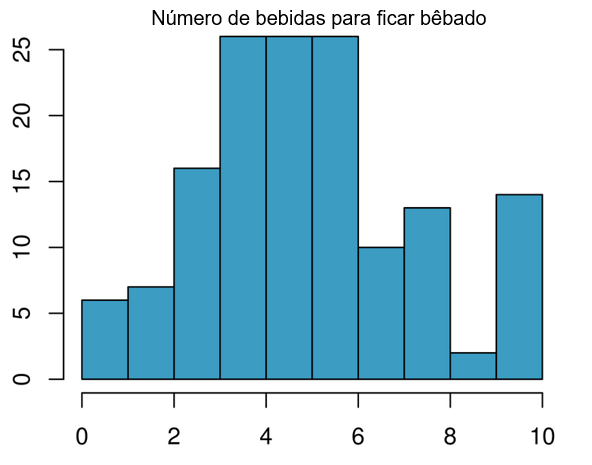
\includegraphics[width=0.4\textwidth]{4-1_var_in_est/no_drinks_drunk.png} 
\end{center}

\end{frame}

%%%%%%%%%%%%%%%%%%%%%%%%%%%%%%%%%%



\begin{frame}[fragile]
\frametitle{Exercício de aplicação}

\begin{center}
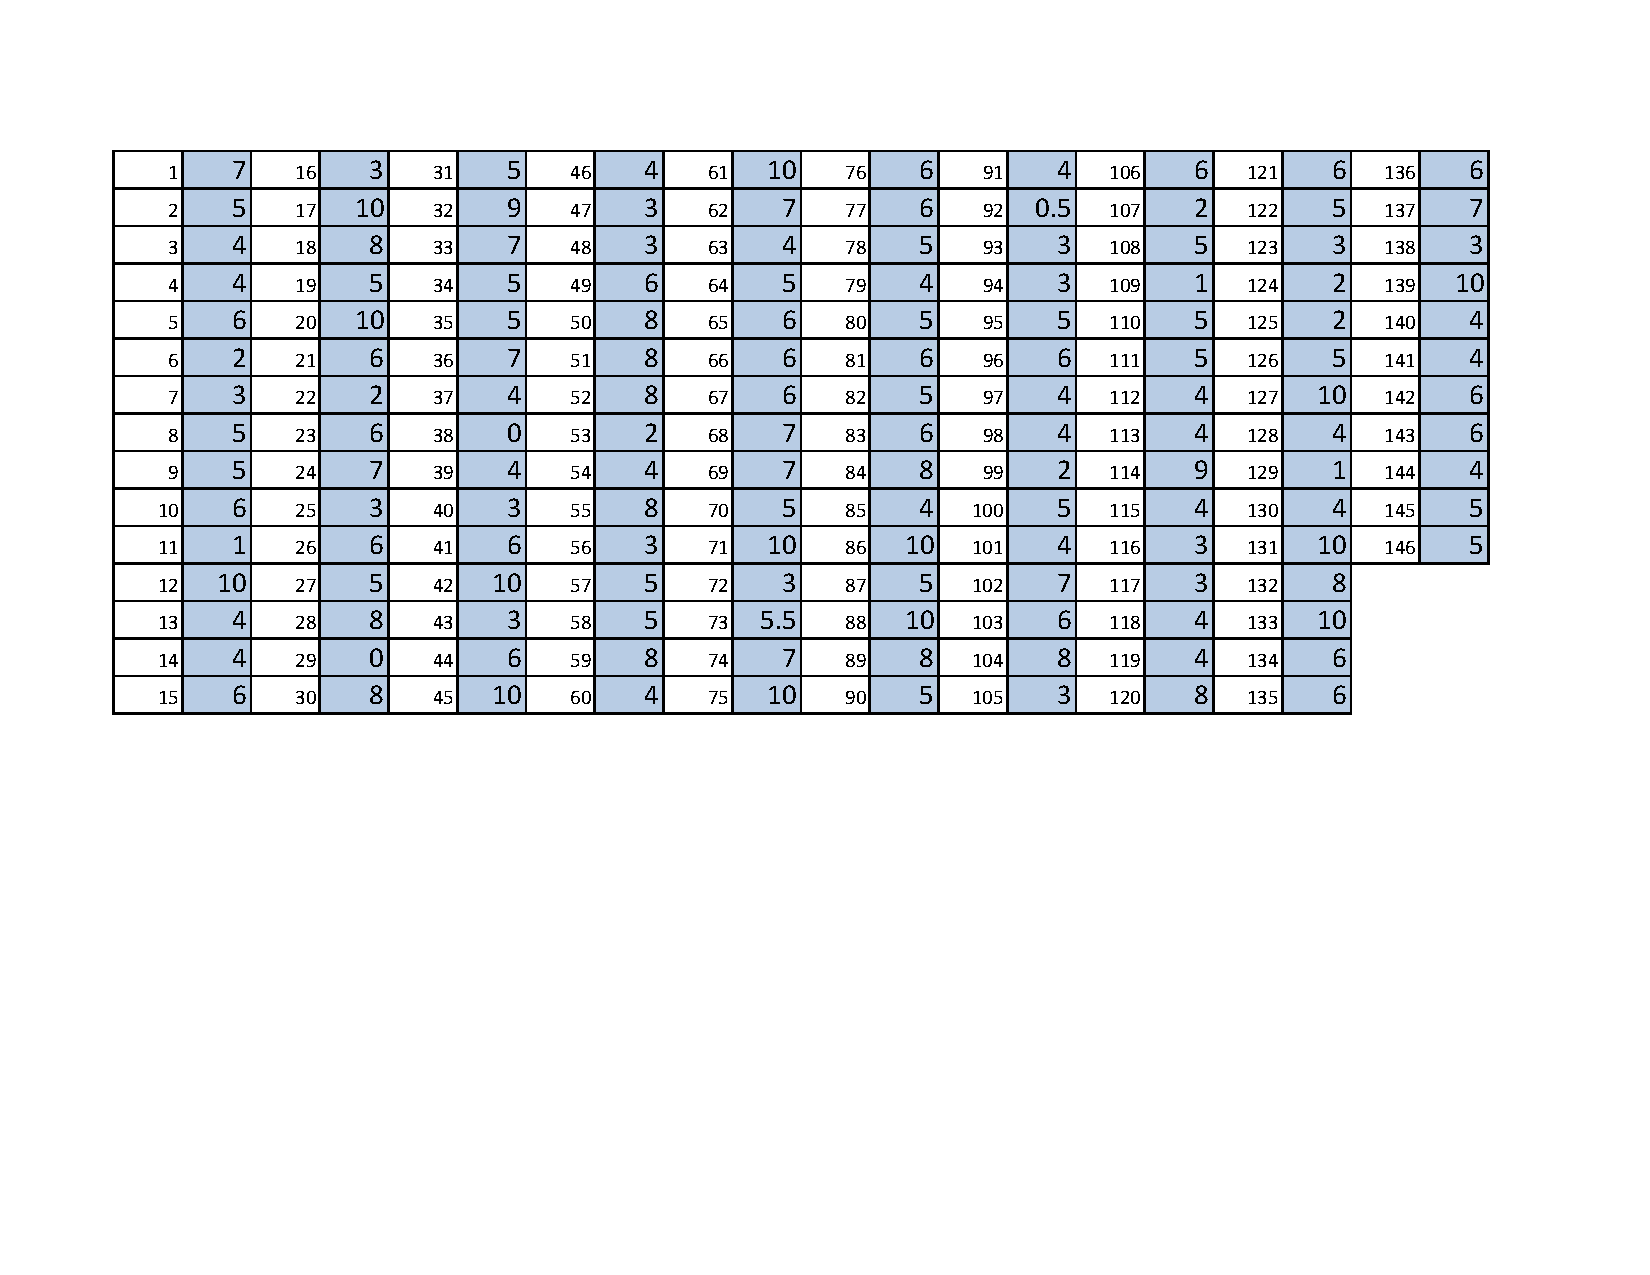
\includegraphics[width=1.05\textwidth]{4-1_var_in_est/no_drinks_drunk_clean.pdf} 
\end{center}

\end{frame}

%%%%%%%%%%%%%%%%%%%%%%%%%%%%%%%%%%%

\begin{frame}[fragile]
\frametitle{Exercício de aplicação}
\justifying
\dq{Exemplo:} Lista de números aleatórios: 59, 121,  88,  46,  58,  72,  82,  81,   5,  10 \\

\begin{center}
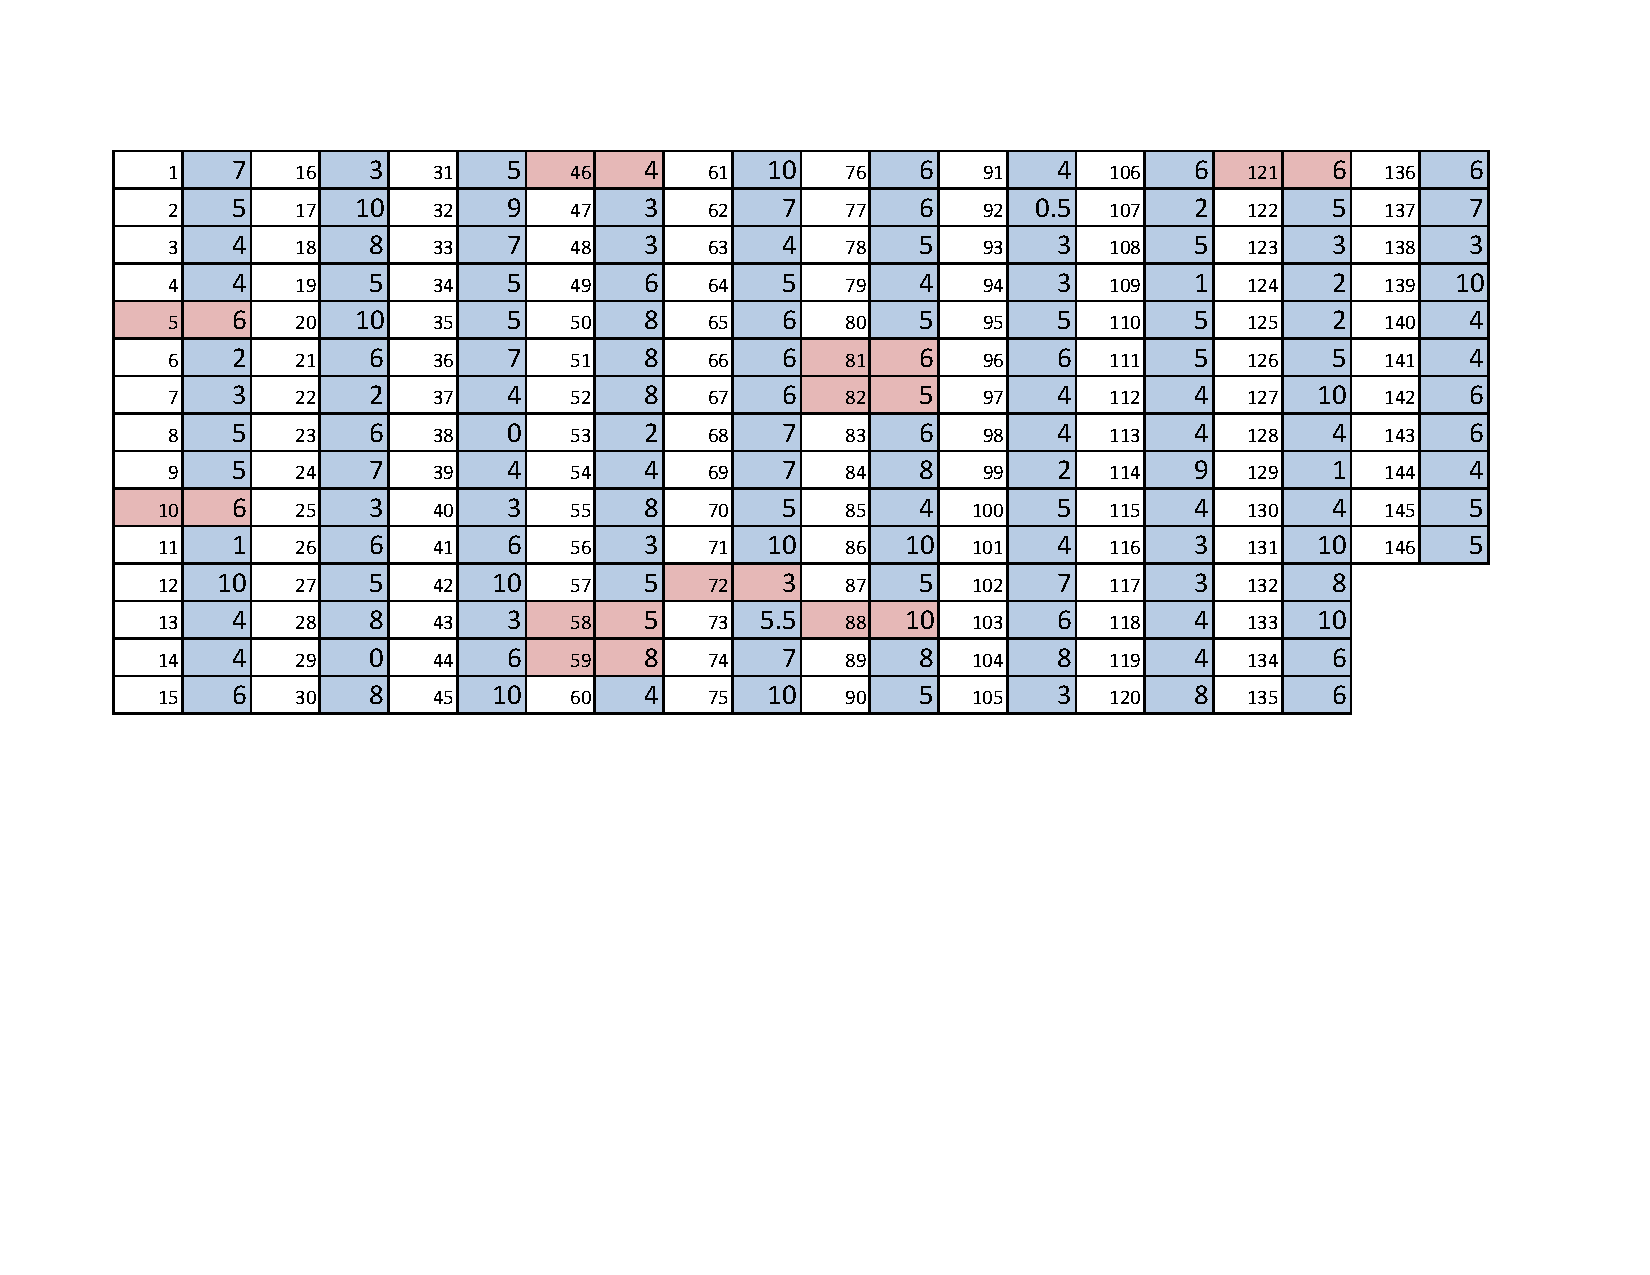
\includegraphics[width=0.9\textwidth]{4-1_var_in_est/no_drinks_drunk_marked.pdf} 
\end{center}

\pause
\justifying
Média da amostra: (8+6+10+4+5+3+5+6+6+6) / 10 = 5.9

\end{frame}

%%%%%%%%%%%%%%%%%%%%%%%%%%%%%%%%%


\begin{frame}[fragile]
\frametitle{Distribuição de amostragem}
\justifying
O que você acabou de construir é chamado de \hl{distribuição de amostragem}.

\pause

$\:$ \\
\justifying
\dq
{Qual é a forma e o centro dessa distribuição? Com base nessa distribuição, qual você acha que é a média real da população?}

$\:$ \\
\justifying
\soln{\only<3>{
Aproximadamente 5,39, a verdadeira média da população.
}}

\end{frame}


%%%%%%%%%%%%%%%%%%%%%%%%%%%%%%%%%%

\subsection{Distribuições de amostragem - via CLT}

%%%%%%%%%%%%%%%%%%%%%%%%%%%%%%%%%%

\begin{frame}
\frametitle{Teorema do limite central (TLC)}
\justifying
\formula{Teorema do limite central}
{A distribuição da média da amostra é bem aproximada por um modelo normal:
\[ \bar{x} \sim N \pr{ \text{média} = \mu, SE = \frac{\sigma}{\sqrt{n}} }, \]
onde SE representa \hl{erro padrão}, que é definido como o desvio padrão da distribuição amostral. Se $\sigma$ é desconhecido, use $s$.
}

\begin{itemize}
\justifying
\item Não foi uma coincidência que a distribuição de amostragem que vimos anteriormente fosse simétrica e centralizada na média real da população.
\end{itemize}
\end{frame}

%%%%%%%%%%%%%%%%%%%%%%%%%%%%%%%%%%

\begin{frame}
\frametitle{Teorema do limite central (TLC)}
\begin{itemize}
\justifying
\item Nós não vamos passar por uma prova detalhada do porquê $SE =  \frac{\sigma}{\sqrt{n}}$, mas note que conforme $n$ aumenta, $SE$ diminui. 
\begin{itemize}
\justifying
\item À medida que o tamanho da amostra aumenta, esperaríamos que as amostras produzissem médias de amostras mais consistentes, portanto a variabilidade entre as médias da amostra seria menor.
\end{itemize}

\end{itemize}

\end{frame}

%%%%%%%%%%%%%%%%%%%%%%%%%%%%%%%%%%%%

\begin{frame}
\frametitle{TLC - condições}
\justifying
Certas condições devem ser atendidas para o TCL valer:

\begin{enumerate}
\justifying
\footnotesize
\item \hlGr{Independência:} As observações da amostra devem ser independentes. \\
\justifying
Isso é difícil de verificar, mas é mais provável termos independência 
\begin{itemize}
\footnotesize
\justifying
\item quando amostragem/atribuição aleatória é realizada, e 
\justifying
\item quando é feita amostragem sem reposição, $n$ $<$ 10\% da população.
\end{itemize}

\pause
\justifying
\item \hlGr{Tamanho da amostra/assimetria:} A distribuição da população é normal ou, se a distribuição da população for assimétrica, o tamanho da amostra precisa ser grande.\\

\begin{itemize}
\footnotesize
\justifying
\item Quanto mais assimétrica a distribuição da população, maior o tamanho da amostra que precisamos para a aplicar TCL.
\justifying
\item para distribuições moderadamente assimétrica $n > 30$ é uma regra prática amplamente usada \\
\end{itemize}

Isso também é difícil de verificar para a população, mas podemos verificá-la usando os dados da amostra e assumir que a amostra espelha a população.

\end{enumerate}
\end{frame}


%%%%%%%%%%%%%%%%%%%%%%%%%%%%%%%%%%%%

\section{4.2. Intervalos de confiança}

%%%%%%%%%%%%%%%%%%%%%%%%%%%%%%%%%%%%

\subsection{Por que relatamos intervalos de confiança?}

%%%%%%%%%%%%%%%%%%%%%%%%%%%%%%%%%%%%

\begin{frame}
\frametitle{Intervalos de confiança}
\footnotesize
\begin{itemize}
\justifying
\item Um intervalo de valores plausível para um parâmetro da população é chamado de \hl{intervalo de confiança}.
\justifying
\item Usar apenas uma estatística de amostra para estimar um parâmetro é como pescar em um lago escuro com uma lança, mas usar um intervalo de confiança é como pescar com uma rede.
$\:$ \\
$\:$ \\
\begin{columns}[c]
\column{0.25\textwidth}
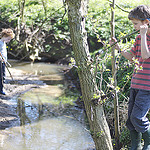
\includegraphics[width=\textwidth]{4-2_conf_int/spear.jpg}
\column{0.5\textwidth}
\justifying
{\footnotesize
Podemos jogar uma lança onde vimos um peixe, mas provavelmente o perderemos. Se atirarmos uma rede nessa área, temos uma boa chance de pegar o peixe.
}
\column{0.25\textwidth}
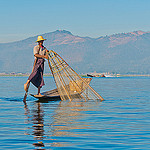
\includegraphics[width=\textwidth]{4-2_conf_int/net.jpg}
\end{columns}
$\:$ \\

\item Se utilizarmos apenas uma estimativa pontual, provavelmente não atingiremos o parâmetro populacional exato. Se utilizarmos um intervalo de valores plausíveis, temos uma boa chance de alçancar o parâmetro.

\end{itemize}

{\tiny Photos by Mark Fischer (http://www.flickr.com/photos/fischerfotos/7439791462) and Chris Penny (http://www.flickr.com/photos/clearlydived/7029109617) on Flickr.}\\

\end{frame}


%%%%%%%%%%%%%%%%%%%%%%%%%%%%%%%%%%%%

\subsection{Construindo um intervalo de confiança}

%%%%%%%%%%%%%%%%%%%%%%%%%%%%%%%%%%%%

\begin{frame}
\frametitle{Número médio de relacionamentos exclusivos}
\justifying
\dq{Uma amostra aleatória de 50 estudantes universitários foi questionada sobre quantos relacionamentos exclusivos eles mantinham até então. Esta amostra rendeu uma média de 3,2 e um desvio padrão de 1,74. Estime o verdadeiro número médio de relacionamentos exclusivos usando essa amostra.}

\pause 

\vspace{-0.5cm}
\[ \bar{x} = 3.2 \qquad s = 1.74 \]

\pause
\justifying
O intervalo de confiança aproximado de 95\% é definido como
\[ estimativa ~ pontual \pm 2 \times SE \]

\pause

\vspace{-0.25cm}
\[ SE = \frac{s}{\sqrt{n}} = \frac{1.74}{\sqrt{50}} \approx 0.25 \]

\end{frame}

%%%%%%%%%%%%%%%%%%%%%%%%%%%%%%%%%%%%%%%%%%%

\begin{frame}
\frametitle{Número médio de relacionamentos exclusivos}

\vspace{-0.25cm}
\begin{eqnarray*}
\bar{x} \pm 2 \times SE &=& 3.2 \pm 2 \times 0.25 \\
\pause
&=& (3.2 - 0.5, 3.2 + 0.5) \\
\pause
&=& (2.7, 3.7)
\end{eqnarray*}


\end{frame}

%%%%%%%%%%%%%%%%%%%%%%%%%%%%%%%%%%%

\begin{frame}
\frametitle{Prática}
\justifying
\pq{Qual das seguintes interpretações deste intervalo de confiança é a correta?}
\justifying
Estamos 95\% confiantes de que
\begin{enumerate}[(a)]
\justifying
\item o número médio de relacionamentos exclusivos que os estudantes universitários da amostra estiveram é entre 2,7 e 3,7.
\justifying
\solnMult{Em média, os estudantes universitários têm entre 2,7 e 3,7 relacionamentos exclusivos.}
\justifying
\item um estudante universitário escolhido aleatoriamente tem de 2,7 a 3,7 relacionamentos exclusivos.
\justifying
\item 95\% dos estudantes universitários têm de 2,7 a 3,7 relacionamentos exclusivos.
\end{enumerate}

\end{frame}

%%%%%%%%%%%%%%%%%%%%%%%%%%%%%%%%%%%

\subsection{Um intervalo mais preciso}

%%%%%%%%%%%%%%%%%%%%%%%%%%%%%%%%%%%

\begin{frame}
\frametitle{Um intervalo mais preciso}
\justifying
\formula{Intervalo de confiança, uma fórmula geral}
{\[ estimativa ~ pontual \pm z^\star \times SE \] }

\pause
\justifying
Condições para ter uma estimação pontual = $\bar{x}$:
\begin{enumerate}
\justifying
\item \hlGr{Independência:} As observações na amostra devem ser independentes
\begin{itemize}
\justifying
\item amostragem/atribuição aleatória
\justifying
\item se amostragem sem reposição, $n <$ 10\% da população
\end{itemize}
\justifying
\item \hlGr{Tamanho da amostra/assimetria:} $ n \ge 30 $ e a distribuição da população não deve ser extremamente assimétrica.

\end{enumerate}

$\:$ \\
\pause
\justifying
{\tiny
\orange{Nota:} Vamos discutir sobre amostras onde $ n <30 $ no próximo capítulo.}

\end{frame}

%%%%%%%%%%%%%%%%%%%%%%%%%%%%%%%%%%%%

\subsection{Capturando o parâmetro populacional}

%%%%%%%%%%%%%%%%%%%%%%%%%%%%%%%%%%%

\begin{frame}
\frametitle{O que significa 95\% de confiança?}

\begin{itemize}
\justifying
\item Suponha que tiramos muitas amostras e construímos um intervalo de confiança de cada amostra usando a equação: \\ {\[ estimativa ~ pontual \pm z^\star \times SE \] }
\justifying
\item Então, cerca de 95\% desses intervalos conteriam a média real da população ($\mu$). 

\end{itemize}

\twocol{0.5}{0.5}
{
\begin{itemize}
\justifying
\footnotesize
\item A figura mostra esse procedimento com 25 amostras, em que 24 dos intervalos de confiança resultantes contém o número médio real de relacionamentos exclusivos e um intervalo não contém o número médio real.

\end{itemize}
}
{
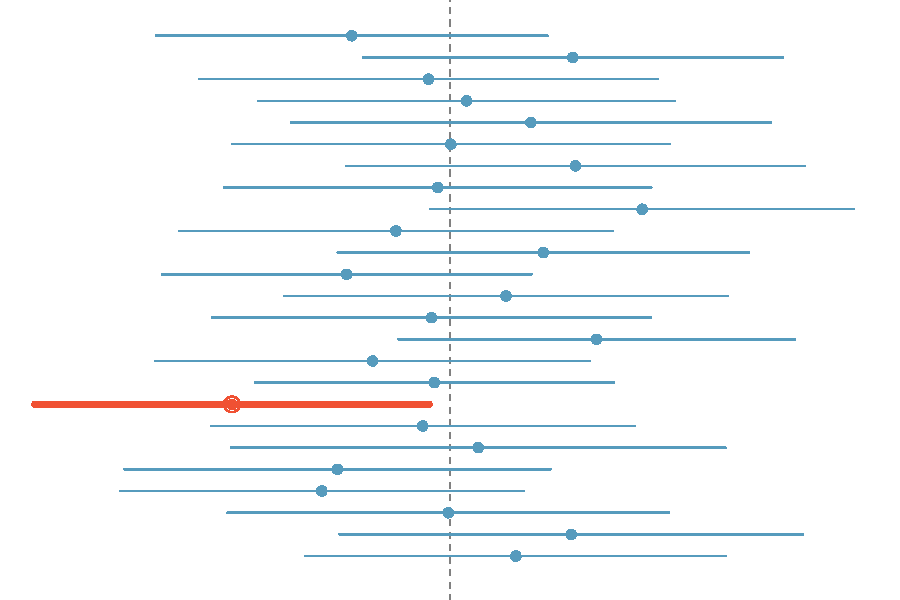
\includegraphics[width=\textwidth]{4-2_conf_int/95PercentConfidenceInterval.pdf}
}

\end{frame}

%%%%%%%%%%%%%%%%%%%%%%%%%%%%%%%%%%%

\begin{frame}
\frametitle{Largura de um intervalo}
\justifying
\dq{Se queremos ter mais certeza de que capturamos o parâmetro população, ou seja, se queremos aumentar o nosso nível de confiança, devemos usar um intervalo maior ou um intervalo menor?}

\pause

\soln{Um intervalo maior.}

$\:$ \\

\pause
\justifying
\dq{Você consegue ver alguma desvantagem em usar um intervalo maior?}
\begin{center}
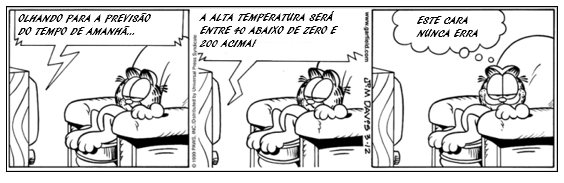
\includegraphics[width=0.6\textwidth]{4-2_conf_int/garfield.png}
\end{center}

\pause
\justifying
\soln{Se o intervalo for muito largo, pode não ser muito informativo.}\\
\justifying
{\scriptsize Image source: http://web.as.uky.edu/statistics/users/earo227/misc/garfield\_weather.gif}

\end{frame}



%%%%%%%%%%%%%%%%%%%%%%%%%%%%%%%%%%%

\subsection{Alterando o nível de confiança}

%%%%%%%%%%%%%%%%%%%%%%%%%%%%%%%%%%%

\begin{frame}
\frametitle{Alterando o nível de confiança}
\justifying
\[ estimativa~pontual\pm z^\star \times SE \] 

\begin{itemize}
\justifying
\item Em um intervalo de confiança, $z ^ \star \times SE $ é chamado de \hl {margem de erro} e, para uma determinada amostra, a margem de erro é alterada conforme o nível de confiança é alterado.
\justifying
\item Para alterar o nível de confiança, precisamos ajustar $ z ^ \star $ na fórmula acima.
\justifying
\item Os níveis de confiança comumente usados são 90\%, 95\%, 98\% e 99\%.
\justifying
\item Para um intervalo de confiança de 95\%, $ z ^ \star = 1.96 $.
\justifying
\item No entanto, usando a distribuição normal padrão ($ z $), é possível encontrar o $ z ^ \star $ apropriado para qualquer nível de confiança.

\end{itemize}

\end{frame}

%%%%%%%%%%%%%%%%%%%%%%%%%%%%%%%%%%%%

\begin{frame}
\frametitle{Prática}
\justifying
\pq{Qual dos valores abaixo de Z é o $z ^ \star $ apropriado ao calcular um intervalo de confiança de 98\%?}

\begin{multicols}{2}
\begin{enumerate}[(a)]
\item $Z = 2.05$
\item $Z = 1.96$
\solnMult{$Z = 2.33$}
\item $Z = -2.33$
\item $Z = -1.65$
\item[]
\end{enumerate}
\end{multicols}


\begin{center}
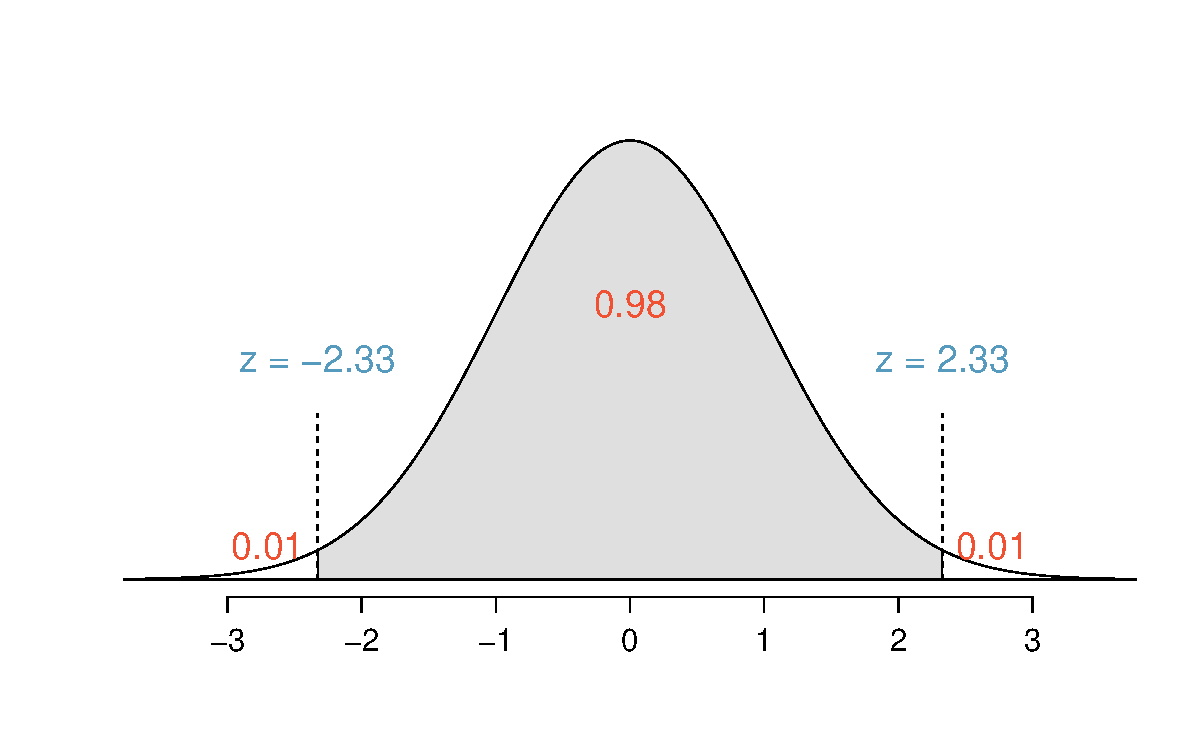
\includegraphics[width=0.7\textwidth]{4-2_conf_int/middle98.pdf}
\end{center}


\end{frame}

%%%%%%%%%%%%%%%%%%%%%%%%%%%%%%%%%%%


%%%%%%%%%%%%%%%%%%%%%%%%%%%%%%%%%%%%

\section{4.3. Testando hipóteses}

%%%%%%%%%%%%%%%%%%%%%%%%%%%%%%%%%%%%

\subsection{Quadro de testes de hipóteses}

%%%%%%%%%%%%%%%%%%%%%%%%%%%%%%%%%%%%

\begin{frame}
\frametitle{Lembre-se de quando...}
\justifying
Experimento sobre discriminação de gênero:
Ser promovido no emprego independe do gênero?

{\small
\begin{tabular}{ll  cc c} 
  		&				& \multicolumn{2}{c}{\textit{Promoção}} \\
\cline{3-4}
							&			& Promovido	& Não Promovido	& Total	\\
\cline{2-5}
\multirow{2}{*}{\textit{Gênero	}}	&Masculino 		& 21	 	& 3		& 24 	\\
							&Feminino		& 14	 	& 10 	 	& 24 \\
\cline{2-5}
							&Total		& 35		& 13		& 48 \\
\end{tabular}
}

\pause
\justifying
\[ \hat{p}_{homens} = 21 / 24 \approx 0.88 \]
\justifying
\[ \hat{p}_{mulheres} = 14 / 24 \approx 0.58 \]

\pause
\end{frame}
%%%%%%%%%%%%%%%%%%%%%%%%%%%%%%%%%%%%

\begin{frame}
\frametitle{Lembre-se de quando...}
Explicações possíveis:
\begin{itemize}
\justifying
\item Promoção e gênero são \hl{independentes}, não há discriminação de gênero, a diferença observada nas proporções é simplesmente devido ao acaso. $\rightarrow$ \orange{nulo} - {\small (nada está acontecendo)}
\justifying
\item Promoção e gênero são \hl{dependentes}, há discriminação de gênero, a diferença observada nas proporções não se deve ao acaso. $\rightarrow$ \orange{alternativa} - {\small (algo está acontecendo)}

\end{itemize}

\end{frame}

%%%%%%%%%%%%%%%%%%%%%%%%%%%%%%%%%%%%

\begin{frame}
\frametitle{Resultado}

\begin{center}
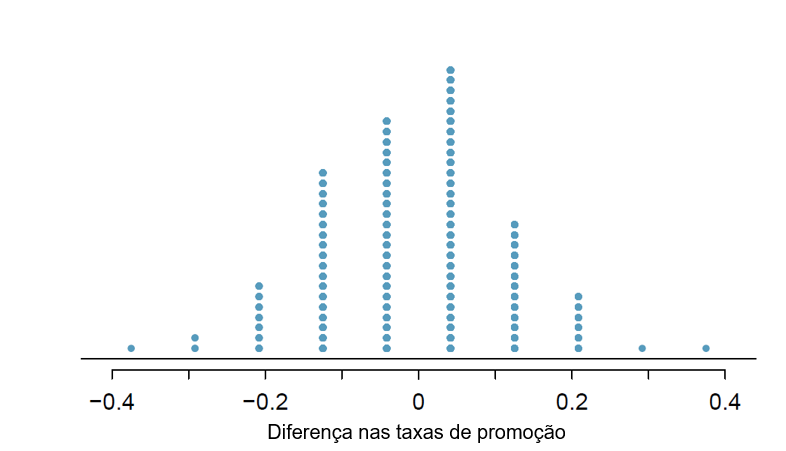
\includegraphics[width=0.6\textwidth]{4-3_hyp_test/discRandDotPlot.png}
\end{center}

\pause
\justifying
Como era bastante improvável obter resultados como os dados reais ou algo mais extremo nas simulações (promoções masculinas sendo 30\% ou mais frequentes às promoções femininas), decidimos rejeitar a hipótese nula em favor da alternativa.

\end{frame}

%%%%%%%%%%%%%%%%%%%%%%%%%%%%%%%%%%%%

\begin{frame}
\frametitle{Recapitulação: estrutura de teste de hipóteses}

\begin{itemize}
\justifying
\item Começamos com uma \hl{hipótese nula ($ H_0 $)} que representa o status quo.
\pause
\justifying
\item Também temos uma hipótese \hl{alternativa ($ H_A $)} que representa nossa questão de pesquisa, ou seja, o que estamos testando.
\pause
\justifying
\item Realizamos um teste de hipóteses sob o pressuposto de que a hipótese nula é verdadeira, seja através de simulação ou métodos tradicionais baseados no teorema do limite central (veremos logo mais...).
\end{itemize}
\end{frame}

%%%%%%%%%%%%%%%%%%%%%%%%%%%%%%%%%%%%

\begin{frame}
\frametitle{Recapitulação: estrutura de teste de hipóteses}

\begin{itemize}
\justifying
\item Se os resultados do teste sugerirem que os dados não fornecem evidências convincentes para a hipótese alternativa, nós ficaremos com a hipótese nula. Mas se o fizerem, rejeitamos a hipótese nula em favor da alternativa.
\end{itemize}
\pause
\justifying
Vamos introduzir formalmente a estrutura de testes de hipóteses usando um exemplo para testar uma afirmação sobre uma média populacional.

\end{frame}

%%%%%%%%%%%%%%%%%%%%%%%%%%%%%%%%%%%%

\subsection{Testando hipóteses usando intervalos de confiança} 

%%%%%%%%%%%%%%%%%%%%%%%%%%%%%%%%%%%%

\begin{frame}
\frametitle{Testando hipóteses usando intervalos de confiança}
\justifying
\dq{Anteriormente, calculamos um intervalo de confiança de 95\% para o número médio de relacionamentos exclusivos em que os estudantes universitários estiveram (2,7, 3,7). Com base nesse intervalo de confiança, esses dados confirmam a hipótese de que os estudantes universitários, em média, já estiveram em mais de três relacionamentos exclusivos.}

\pause

\begin{itemize}
\justifying
\item As hipóteses associadas são:
\begin{itemize}
\justifying
\item[$H_0$:] $\mu = 3$: Os estudantes universitários já estiveram em três relacionamentos exclusivos, em média.
\justifying
\item[$H_A$:] $\mu > 3$: Os estudantes universitários já estiveram em mais de 3 relacionamentos exclusivos, em média.
\end{itemize}
\end{itemize}

\end{frame}
%%%%%%%%%%%%%%%%%%%%%%%%%%%%%%%%%%%%

\begin{frame}
\frametitle{Testando hipóteses usando intervalos de confiança}

\begin{itemize}
\justifying
\item Como o valor nulo está dentro do intervalo, não rejeitamos a hipótese nula em favor da alternativa.

\pause
\justifying
\item Esta é uma abordagem rápida (e um pouco tosca) para fazer testes de hipóteses. No entanto, ela não nos diz a probabilidade de certos resultados sob a hipótese nula, ou seja, o p-valor, com base no qual podemos tomar uma decisão sobre as hipóteses.

\end{itemize}

\end{frame}

%%%%%%%%%%%%%%%%%%%%%%%%%%%%%%%%%%%%

\begin{frame}
\frametitle{Número de pedidos de faculdade}
\justifying
\dq{{\small Uma pesquisa semelhante perguntou para 206 alunos da Duke University para quantas faculdades eles aplicaram. Esta amostra rendeu uma média de 9,7 aplicações universitárias com um desvio padrão de 7. O site do College Board afirma que os orientadores recomendam que os alunos se inscrevam em aproximadamente 8 faculdades. Esses dados fornecem evidências convincentes de que o número médio de faculdades aos quais os alunos da Duke se candidatam é \emph{superior} ao recomendado?}}

\vfill
\justifying
\ct{\webURL{http://www.collegeboard.com/student/apply/the-application/151680.html}}

\end{frame}

%%%%%%%%%%%%%%%%%%%%%%%%%%%%%%%%%%

\begin{frame}
\frametitle{Definindo as hipóteses}

\begin{itemize}
\justifying
\item O \hl{parâmetro de interesse} é o número médio de escolas aplicadas por \underline{todos} estudantes da Duke.

\pause
\justifying
\item Pode haver duas explicações para a nossa média de amostra ser maior do que as 8 faculdades recomendadas.
\begin{itemize}
\justifying
\item A verdadeira média populacional é diferente.
\justifying
\item A média real da população é 8, e a diferença entre a média real da população e a média da amostra é simplesmente devido à variabilidade natural da amostragem.
\end{itemize}

\pause
\end{itemize}

\end{frame}
%%%%%%%%%%%%%%%%%%%%%%%%%%%%%%%%%%

\begin{frame}
\frametitle{Definindo as hipóteses}

\begin{itemize}
\justifying
\item Começamos com a suposição de que o número médio de faculdades em que os alunos da Duke se candidatam é 8 (como recomendado)
\[ \mathhl{H_0:}~\mu = 8 \]

\pause
\justifying
\item Testamos a alegação de que o número médio de faculdades em que os alunos da Duke se candidatam é maior que 8
\[ \mathhl{H_A:}~\mu > 8 \]

\end{itemize}

\end{frame}

%%%%%%%%%%%%%%%%%%%%%%%%%%%%%%%%%%%

\subsection{Condições para inferência}

%%%%%%%%%%%%%%%%%%%%%%%%%%%%%%%%%%%

\begin{frame}
\frametitle{Número de candidaturas universitárias - condições}
\justifying
\pq{Qual das seguintes opções \emph{não} é uma condição que precisa ser atendida para aplicar este teste de hipótese?}

\begin{enumerate}[(a)]
\justifying
\item Os alunos da amostra devem ser independentes uns dos outros em relação a quantas faculdades se candidataram.
\justifying
\item A amostragem deveria ter sido feita aleatoriamente.
\justifying
\item O tamanho da amostra deve ser menor que 10 \% da população de todos os alunos da Duke.
\justifying
\solnMult{ Deve haver pelo menos 10 sucessos e 10 falhas na amostra.}
\justifying
\item A distribuição do número de faculdades em que os alunos aplicaram não deve ser extremamente assimétrica.
\end{enumerate}

\end{frame}

%%%%%%%%%%%%%%%%%%%%%%%%%%%%%%%%%%

\subsection{Teste formal usando valores p}

%%%%%%%%%%%%%%%%%%%%%%%%%%%%%%%%%%%%

\begin{frame}
\frametitle{Estatística de teste}
\justifying
Para avaliar se a média da amostra observada é diferente da distribuição de amostragem hipotética, determinamos quantos erros-padrão podem estar fora da hipótese nula, o que também é chamado de \hl{estatística de teste}.


\pause

\twocol{0.55}{0.45}{
\begin{center}
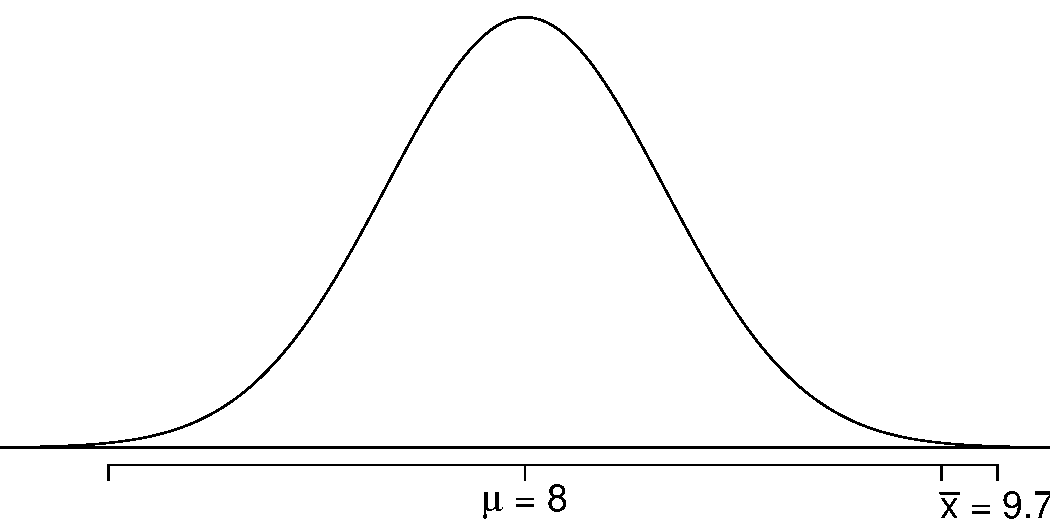
\includegraphics[width=\textwidth]{4-3_hyp_test/app_z.pdf}
\end{center}
\pause
\[ \bar{x} \sim N \pr{ \mu = 8, SE = \frac{7}{\sqrt{206}} = 0.5 } \]
\pause
\[ Z = \frac{9.7 - 8}{0.5} = 3.4 \]
}
{
\pause
\justifying
\tiny{\dq{A média da amostra é de 3,4 erros padrão longe do valor hipotético. Isso é considerado excepcionalmente alto? Ou seja, é o resultado \hl{estatisticamente significativo}?}
\pause
\justifying
\soln{Sim, e podemos quantificar o quão incomum é essa média usando um p-valor.}
}}

\end{frame}

%%%%%%%%%%%%%%%%%%%%%%%%%%%%%%%%%%%

\begin{frame}
\frametitle{P-valor}

\begin{itemize}
\justifying
\item Em seguida, usamos essa estatística de teste para calcular o \hl{p-valor}, ou seja, a probabilidade de observar dados tão favoráveis à hipótese alternativa quanto nosso conjunto de dados atual, se a hipótese nula fosse verdadeira.


\pause
\justifying
\item Se o p-valor for \hl{baixo} (menor que o nível de significância, $\alpha$, que normalmente é de 5\%), dizemos que seria muito improvável observar os dados se a hipótese nula fosse verdadeira, e daí \hl{rejeitamos $H_0$}.

\pause
\justifying
\item Se o p-valor for \hl{alto} (maior que $\alpha$), dizemos que é provável observar os dados mesmo que a hipótese nula seja verdadeira e, portanto, \hl{não rejeitamos $H_0$}.

\end{itemize}

\end{frame}

%%%%%%%%%%%%%%%%%%%%%%%%%%%%%%%%%%%%

\begin{frame}
\frametitle{Número de inscrições em faculdades - p-valor}
\justifying
\hl{P-valor:} probabilidade de observar dados pelo menos tão favoráveis a $H_A$ como nosso conjunto de dados atual (uma média de amostra maior que 9,7), se de fato $H_0$ fosse verdadeira (a média real da população é 8).


\begin{center}
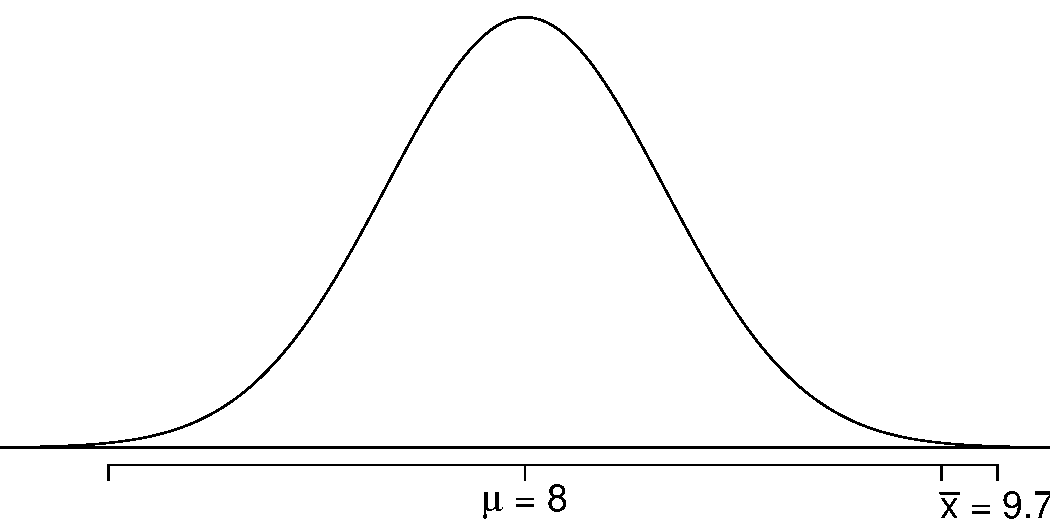
\includegraphics[width=0.55\textwidth]{4-3_hyp_test/app_pval_gr.pdf}
\end{center}

\pause

\[ P(\bar{x} > 9.7~|~\mu = 8) = P(Z > 3.4) = 0.0003 \]

\end{frame}

%%%%%%%%%%%%%%%%%%%%%%%%%%%%%%%%%%

\begin{frame}
\frametitle{Número de inscrições em faculdades - tomada de decisão}

\begin{itemize}
\justifying
\item p-valor = 0.0003

\pause

\begin{itemize}
\justifying
\item Se a média real do número de faculdades em que os alunos da Duke se candidataram é 8, há apenas 0,03\% de chance de observar uma amostra aleatória de 206 alunos da Duke que, em média, aplicaram para 9,7 ou mais faculdades.

\pause
\justifying
\item Esta é uma probabilidade muito baixa para acreeditarmos que uma média amostral de 9,7 ou mais faculdades acontecerá por acaso.
\end{itemize}

\pause
\justifying
\item Como o p-valor é \orange{baixo} (menor que 5\%), nós \orange {rejeitamos $H_0$}.

\pause
\justifying
\item Os dados fornecem evidências convincentes de que os alunos da Duke aplicaram para mais de 8 faculdades, em média.

\pause
\justifying
\item A diferença entre o a hipótese nula de 8 faculdades e a média amostral observada de 9,7 faculdades \orange{não é por acaso} ou devido à variabilidade amostral.

\end{itemize}

\end{frame}

%%%%%%%%%%%%%%%%%%%%%%%%%%%%%%%%%%%%

\begin{frame}
\frametitle{Prática}
\justifying
\pq{ Uma pesquisa da National Sleep Foundation descobriu que os estudantes universitários têm em média 7 horas de sono por noite. Uma amostra de 169 estudantes universitários que fizeram uma aula de estatística introdutória rendeu uma média de 6,88 horas de sono por noite, com um desvio padrão de 0,94 horas. Supondo que esta seja uma amostra aleatória representativa de todos os estudantes universitários {\scriptsize \textit{(com um pouco de fé?)}}, um teste de hipótese foi realizado para avaliar se os estudantes universitários em média dormem \emph{menos que} 7 horas por noite. O p-valor para este teste de hipótese é 0,0485. Qual das seguintes opções está correta?}
\end{frame}
%%%%%%%%%%%%%%%%%%%%%%%%%%%%%%%%%%%%%%%
\begin{frame}
\frametitle{Prática}
\begin{enumerate}[(a)]
\justifying
\item Não rejeitamos $H_0$, os dados fornecem evidências convincentes de que os estudantes universitários dormem em média menos de 7 horas.
\justifying
\solnMult{ Rejeitamos $H_0$, os dados fornecem evidências convincentes de que os estudantes universitários dormem menos de 7 horas em média. }
\justifying
\item Rejeitamos $H_0$, os dados provam que os estudantes universitários dormem mais de 7 horas em média.
\justifying
\item Não rejeitamos $H_0$, os dados não fornecem evidências convincentes de que os estudantes universitários dormem menos de 7 horas em média.
\justifying
\item Rejeitamos $H_0$, os dados fornecem evidências convincentes de que os estudantes universitários nesta amostra dormem menos de 7 horas em média.
\end{enumerate}

\end{frame}

%%%%%%%%%%%%%%%%%%%%%%%%%%%%%%%%%

\subsection{Teste de hipóteses bilateral e p-valor}

%%%%%%%%%%%%%%%%%%%%%%%%%%%%%%%%%

\begin{frame}
\frametitle{Teste de hipóteses bilateral e p-valor}

\begin{itemize}
\justifying
\item Se a pergunta de pesquisa for "Os dados fornecem evidências convincentes de que a média de sono dos estudantes universitários por noite é \orange{diferente} que a média nacional?", a hipótese alternativa seria diferente.
\begin{align*}
H_0&: \mu = 7 \\
H_A&: \mu \orange{~$\ne$~} 7
\end{align*}

\pause
\justifying
\item Portanto, o p-valor também mudaria:
\twocol{0.55}{0.45}
{
\begin{center}
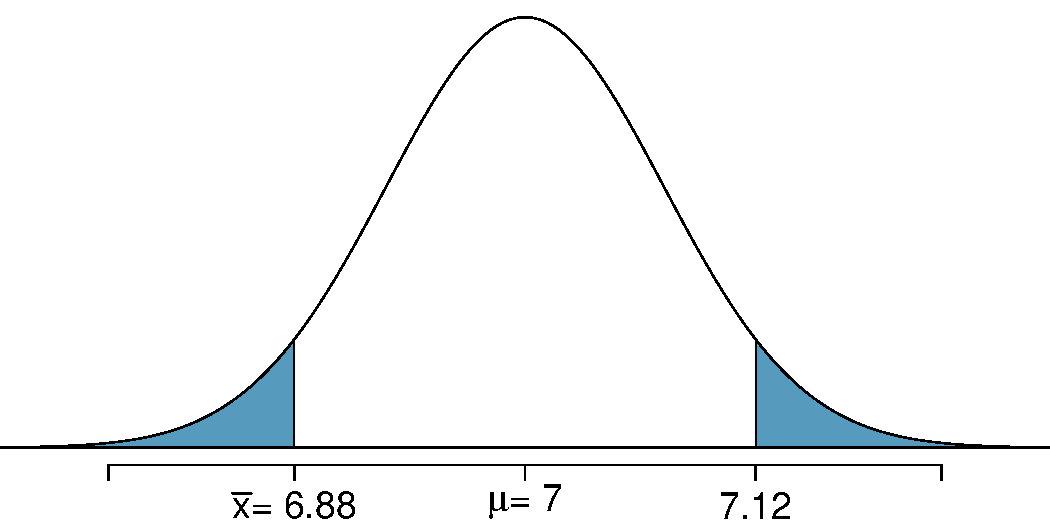
\includegraphics[width=\textwidth]{4-3_hyp_test/sleep_pval_ts.pdf}
\end{center}
}
{
\small{valor-p \\
$= 0.0485 \times 2$ \\
$= 0.097$
}}

\end{itemize}

\end{frame}

%%%%%%%%%%%%%%%%%%%%%%%%%%%%%%%%%%%%

\subsection{Erros de decisão}

%%%%%%%%%%%%%%%%%%%%%%%%%%%%%%%%%%%%

\begin{frame}
\frametitle{Erros de decisão}

\begin{itemize}
\justifying
\item Testes de hipóteses não são perfeitos.
\justifying
\item No sistema judiciário, pessoas inocentes são às vezes erroneamente condenadas e os culpados às vezes saem impunes.
\justifying
\item Da mesma forma, podemos tomar uma decisão errada nos testes de hipóteses estatísticas.
\justifying
\item A diferença é que temos as ferramentas necessárias para quantificar a frequência com que cometemos erros nas estatísticas.

\end{itemize}

\end{frame}

%%%%%%%%%%%%%%%%%%%%%%%%%%%%%%%%%%%%

\begin{frame}
\frametitle{Erros de decisão (cont.)}
\justifying
Existem duas hipóteses concorrentes: a nula e a alternativa. Em um teste de hipótese, tomamos uma decisão sobre o que pode ser verdade, mas nossa escolha pode estar incorreta. \\

\pause

\begin{center}
\begin{tabular}{l l | c c}
\multicolumn{2}{c}{} & \multicolumn{2}{c}{\textbf{Decisão}} \\
& & não rejeitar $H_0$ &  rejeitar $H_0$ \\
  \cline{2-4}
& $H_0$ verdadeiro & \onslide<3->{\green{$\checkmark$}} &  \onslide<5->{\orange{Erro tipo 1}} \\
\raisebox{1.5ex}{\textbf{Verdade}} & $H_A$ verdadeiro & \onslide<6->{\orange{Erro tipo 2}} & \onslide<4->{\green{$\checkmark$}} \\
  \cline{2-4}
\end{tabular}
\end{center}

\begin{itemize}
\justifying
\item \onslide<5->{O \hl{erro tipo 1} é quando rejeitamos a hipótese nula quando, na verdade, $H_0$ é verdadeiro.}
\justifying
\item \onslide<6->{O \hl {erro tipo 2} é quando não conseguimos rejeitar a hipótese nula quando, na verdade, $H_A$ é verdadeiro.}
\justifying
\item \onslide<7->{Nós (quase) nunca sabemos se $H_0$ ou $H_A$ é a verdade, mas precisamos considerar todas as possibilidades.}

\end{itemize}

\end{frame}

%%%%%%%%%%%%%%%%%%%%%%%%%%%%%%%%%%%%

\begin{frame}
\frametitle{Teste de Hipótese como um julgamento}
\justifying
Se pensarmos novamente em um teste de hipótese como um processo criminal, então faz sentido enquadrar o veredito em termos das hipóteses nula e alternativa:
\begin{align*}
H_0&:\text{ Réu é inocente} \\
H_A&:\text{ Réu é culpado}
\end{align*}
\justifying
Qual tipo de erro está sendo cometido nas seguintes circunstâncias?

\begin{itemize}
\justifying
\item Declarando o réu inocente quando ele é culpado.
\justifying
\soln{\only<2->{\begin{center}\hl{Erro tipo 2}\end{center}}}
\justifying
\item Declarando o réu culpado quando ele é inocente.
\justifying
\soln{\only<3->{\begin{center}\hl{Erro tipo 1}\end{center}}}
\end{itemize}
\justifying
\only<4->{Qual erro você acha que é pior?}
\justifying
\only<5>{\begin{center}{\footnotesize ``melhor dez pessoas culpadas escaparem do que um inocente sofrer''\\ -- William Blackstone}\end{center}}
\end{frame}

%%%%%%%%%%%%%%%%%%%%%%%%%%%%%%%%%%%%

\begin{frame}
\frametitle{Taxa de erro de tipo 1}

\begin{itemize}
\justifying
\item Como regra geral, rejeitamos $H_0$ quando o p-valor é menor que 0,05, ou seja, usamos um \hl{nível de significância} de 0,05, \mathhl{\alpha = 0.05}.

\pause
\justifying
\item Isso significa que, nos casos em que $H_0$ é realmente verdadeira, não queremos rejeitá-la incorretamente mais de 5\% dessas vezes. 

\pause
\justifying
\item Em outras palavras, ao usar um nível de significância de 5\%, há cerca de 5\% de chance de gerar um erro de Tipo 1 se a hipótese nula for verdadeira.
\[ \mathhl{ P(\text{Erro tipo 1 | $H_0$ Verdade}) = \alpha } \]

\pause
\justifying
\item É por isso que preferimos valores pequenos de $\alpha$ -- aumentando $\alpha$ aumenta a taxa de erro do tipo 1.

\end{itemize}

\end{frame}

%%%%%%%%%%%%%%%%%%%%%%%%%%%%%%%%%%%%

\subsection{Escolhendo um nível de significância}

%%%%%%%%%%%%%%%%%%%%%%%%%%%%%%%%%%%%

\begin{frame}
\frametitle{Escolhendo um nível de significância}

\begin{itemize}
\justifying
\item Escolher um nível de significância para um teste é importante em muitos contextos, e o nível tradicional é de 0,05. No entanto, geralmente é útil ajustar o nível de significância com base no que se está testando. 
\justifying
\item Podemos selecionar um nível menor ou maior que 0,05, dependendo das consequências de quaisquer conclusões obtidas no teste.
\justifying
\item Se as consequências de um Erro Tipo 1 forem perigosas ou caras, devemos escolher um nível de significância pequeno (por exemplo, 0,01). Sob este cenário, queremos ser muito cautelosos ao rejeitar a hipótese nula, então exigimos evidências muito fortes favorecendo $H_A$ antes de rejeitarmos $H_0$.
\end{itemize}

\end{frame}

%%%%%%%%%%%%%%%%%%%%%%%%%%%%%%%%%%%%

\begin{frame}
\frametitle{Escolhendo um nível de significância}

\begin{itemize}
\justifying
\item Se um Erro Tipo 2 for relativamente mais perigoso ou muito mais dispendioso do que um Erro Tipo 1, então devemos escolher um nível de significância mais alto (por exemplo, 0,10). Aqui, queremos ter cautela ao não rejeitar $H_0$ quando a hipótese nula for realmente falsa.

\end{itemize}

\end{frame}

%%%%%%%%%%%%%%%%%%%%%%%%%%%%%%%%%%%%

\subsection{Recap}

%%%%%%%%%%%%%%%%%%%%%%%%%%%%%%%%%%%%

\begin{frame}

\vfill
\justifying
\textit{As próximas paginas serão um breve resumo dos testes de hipóteses..}

\vfill

\end{frame}

%%%%%%%%%%%%%%%%%%%%%%%%%%%%%%%%%%%%

\begin{frame}
\frametitle{Recapitulação: estrutura de testes de hipóteses}

\begin{enumerate}
\justifying
\item Defina as hipóteses.
\justifying
\item Verifique as suposições e condições.
\justifying
\item Calcule uma \hl {estatística de teste} e um p-valor.
\justifying
\item Tome uma decisão e interprete-a no contexto da questão de pesquisa.

\end{enumerate}

\end{frame}

%%%%%%%%%%%%%%%%%%%%%%%%%%%%%%%%%%%

\begin{frame}
\frametitle{Recapitulação: teste de hipóteses para uma média populacional}

\begin{enumerate}
\justifying
\item Defina as hipóteses
\begin{itemize}
\item $H_0: \mu = valor~nulo$
\item $H_A: \mu <$ ou $>$ ou $\ne valor~nulo$
\end{itemize}
\justifying
\item Calcular a estimativa pontual
\justifying
\item Verifique as suposições e condições
\begin{itemize}
\justifying
\item Independência: amostra/atribuição aleatória, condição de 10\% quando amostragem é sem substituição.
\justifying
\item Normalidade: população quase normal ou $n \ge 30$, sem assimetria extrema - ou use a distribuição t.
\end{itemize}
\justifying
\item Calcule uma \hl{estatística de teste} e um p-valor (desenhe uma figura!)
\[ Z = \frac{\bar{x} - \mu}{SE},~onde~SE = \frac{s}{\sqrt{n}} \]
\justifying
\item Tome uma decisão e interprete-a no contexto
\end{enumerate}

\end{frame}
%%%%%%%%%%%%%%%%%%%%%%%%%%%%%%%%%%%%%%%%%%%%%%%%%%%%%%
\begin{frame}
\frametitle{Recapitulação: teste de hipóteses para uma média populacional}

\begin{itemize}
\justifying
\item Se o p-valor for p $<\alpha$, rejeitamos $H_0$, os dados fornecem evidências à favor de $H_A$.
\justifying
\item Se o p-valor for p $>\alpha$, não rejeitamos $H_0$, os dados não fornecem evidências à favor de $H_A$.
\end{itemize}



\end{frame}

%%%%%%%%%%%%%%%%%%%%%%%%%%%%%%%%%%%%




%%%%%%%%%%%%%%%%%%%%%%%%%%%%%%%%%%%

\section{4.4. Teorema do Limite Central}

%%%%%%%%%%%%%%%%%%%%%%%%%%%%%%%%%%%

\begin{frame}[fragile]
\frametitle{Número médio de jogos de basquete}
\justifying
Em seguida, vamos ver os dados da população para o número de jogos de basquete que assitiram:

\begin{center}
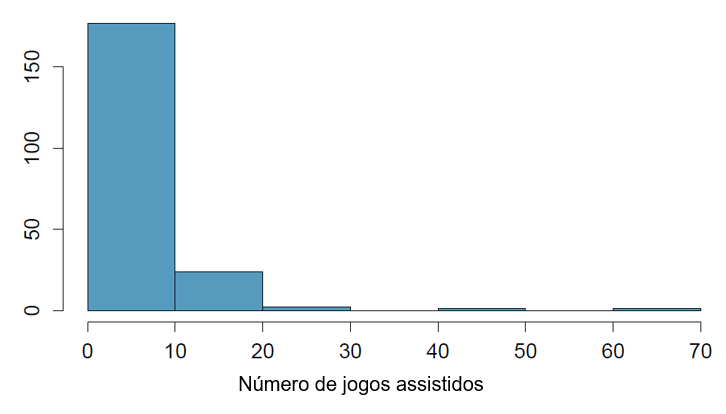
\includegraphics[width=0.8\textwidth]{4-4_clt/duke_games_pop.png}
\end{center}


\end{frame}


%%%%%%%%%%%%%%%%%%%%%%%%%%%%%%%%%%%

\begin{frame}[fragile]
\frametitle{Número médio de jogos de basquete (cont.)}
\justifying
Distribuição de amostras, n = 10:

\twocol{0.6}{0.4}{
\begin{center}
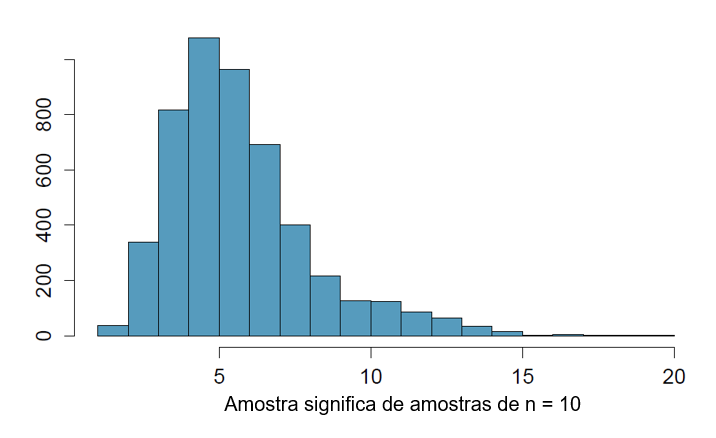
\includegraphics[width=\textwidth]{4-4_clt/duke_games_n10.png}
\end{center}
}
{\justifying
\dq{O que cada observação nesta distribuição representa??}
\justifying
\soln{\only<1>{\textcolor{white}{Média da amostra ($\bar{x}$) de amostras de tamanho $n = 10$.}}}
\justifying
\soln{\only<2->{Média da amostra ($\bar{x}$) de amostras de tamanho $n = 10$.}}

}

\end{frame}
%%%%%%%%%%%%%%%%%%%%%%%%%%%%%%%%%%%

\begin{frame}[fragile]
\frametitle{Número médio de jogos de basquete (cont.)}
\justifying
Distribuição de amostras, n = 10:

\twocol{0.6}{0.4}{
\begin{center}
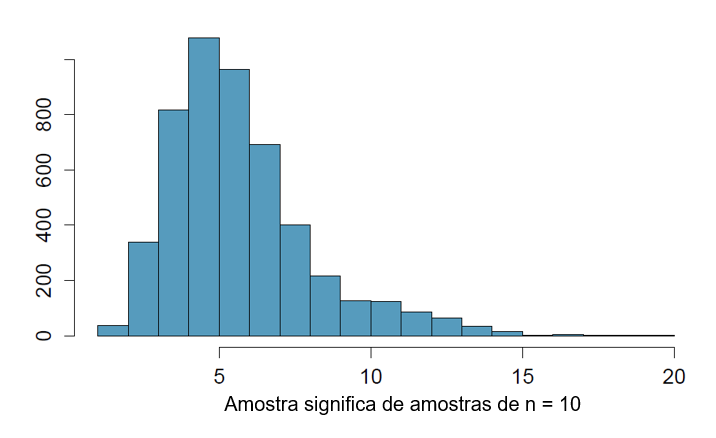
\includegraphics[width=\textwidth]{4-4_clt/duke_games_n10.png}
\end{center}
}
{\justifying
\dq{A variabilidade da distribuição amostral é menor ou maior que a variabilidade da distribuição populacional? Por quê?}
\justifying
\soln{\only<1-2>{\textcolor{white}{Menor, a média das amostras irá variar menos do que as observações individuais.}}}
\justifying
\soln{\only<3->{Menor, a média das amostras irá variar menos do que as observações individuais.}}
}

\end{frame}
%%%%%%%%%%%%%%%%%%%%%%%%%%%%%%%%%%%%

\begin{frame}[fragile]
\frametitle{Número médio de jogos de basquete (cont.)}
\justifying
Distribuição de amostras, n = 30:

\twocol{0.6}{0.4}{
\begin{center}
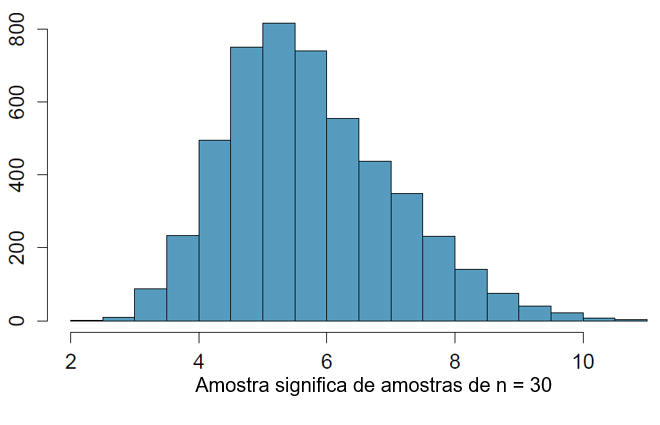
\includegraphics[width=\textwidth]{4-4_clt/duke_games_n30.png}
\end{center}
}
{\justifying
\dq{Como o formato, o centro e a disposição da distribuição amostral mudaram de $n = 10$ para $n = 30$?}
\justifying
\soln{\only<1>{\textcolor{white}{O formato é mais simétrico, o centro é aproximadamente o mesmo, a disposição é menor.}}}
\justifying
\soln{\only<2->{O formato é mais simétrico, o centro é aproximadamente o mesmo, a disposição é menor.}}
}

\end{frame}


%%%%%%%%%%%%%%%%%%%%%%%%%%%%%%%%%%%%

\begin{frame}[fragile]
\frametitle{Número médio de jogos de basquete (cont.)}
\justifying
Distribuição de amostras, n = 70:

\begin{center}
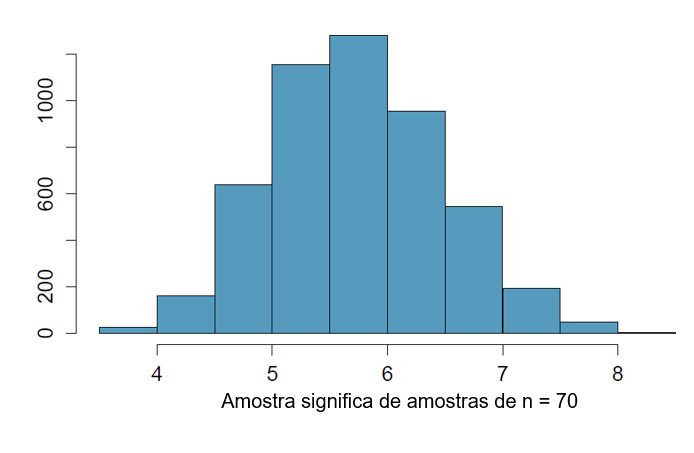
\includegraphics[width=0.6\textwidth]{4-4_clt/duke_games_n70.png}
\end{center}

\end{frame}


%%%%%%%%%%%%%%%%%%%%%%%%%%%%%%%%%%%%

\begin{frame}[fragile]
\frametitle{Número médio de jogos de basquete (cont.)}
\justifying
\dq{A média da distribuição amostral é de 5,75 e o desvio padrão da distribuição amostral (também chamado de \hl{erro padrão}) é 0,75. Qual dos seguintes opções é o palpite mais razoável para o intervalo de confiança de 95\% para o número médio real de jogos de basquete assistidos?}

\begin{enumerate}[(a)]
\item $5.75 \pm 0.75$
\solnMult{$5.75 \pm 2 \times 0.75$} \soln{\only<2>{\red{$\rightarrow (4.25,7.25)$}}}
\item $5.75 \pm 3 \times 0.75$
\item não podemos afirmar nada com as informações dadas.
\end{enumerate}


\end{frame}

%%%%%%%%%%%%%%%%%%%%%%%%%%%%%%%%%%%

\begin{frame}
\frametitle{Prática}
\justifying
\pq{
{ Quatro gráficos: determine qual gráficos (A, B ou C) é qual. \\
(1) No topo: distribuição para uma população ($\mu = 10, \sigma = 7$), \\
(2) uma única amostra aleatória de 100 observações dessa população, \\
(3) uma distribuição de 100 amostras de amostras aleatórias com tamanho 7, e \\
(4) uma distribuição de 100 amostras de amostras aleatórias com tamanho 49.}}

\end{frame}
%%%%%%%%%%%%%%%%%%%%%%%%%%%%%%%%%%%

\begin{frame}
\frametitle{Prática}

\twocol{0.4}{0.6}{
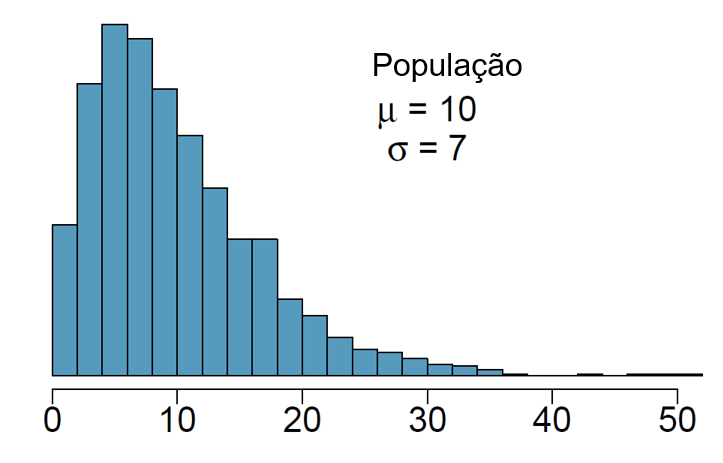
\includegraphics[width=\textwidth]{4-4_clt/cltSimRS_pop.png}
}
{
\vspace{-0.5cm}
{\small
\begin{enumerate}[(a)]
\solnMult{A - (3); B - (2); C - (4)}
\item A - (2); B - (3); C - (4)
\item A - (3); B - (4); C - (2)
\item A - (4); B - (2); C - (3)
\end{enumerate}
}
}
\vspace{-0.25cm}
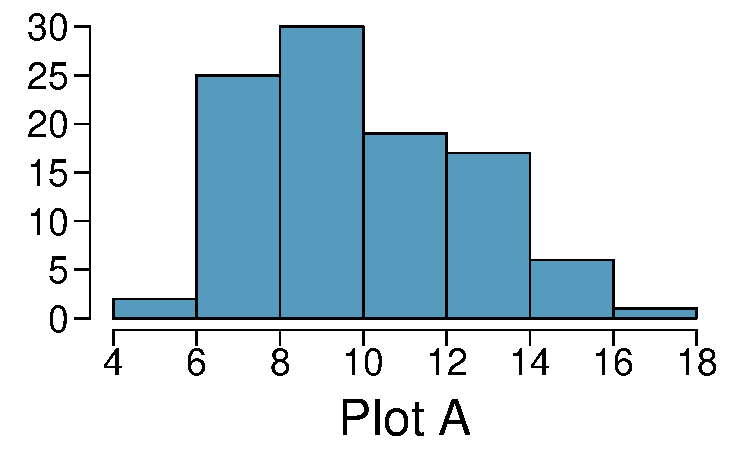
\includegraphics[width=0.32\textwidth]{4-4_clt/cltSimRS_n7.pdf}
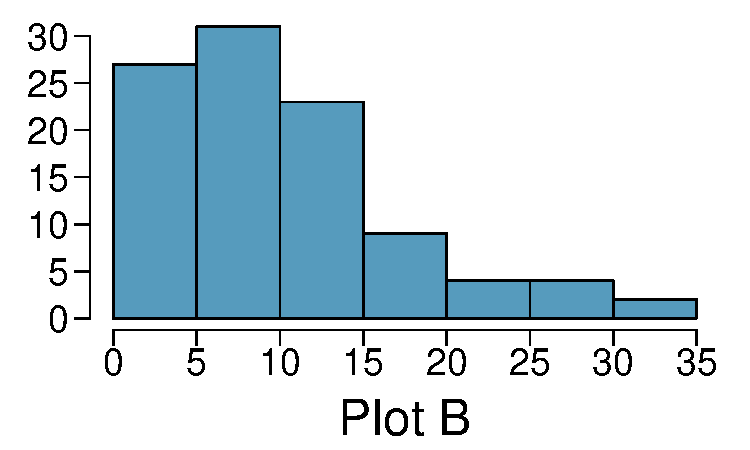
\includegraphics[width=0.32\textwidth]{4-4_clt/cltSimRS_samp.pdf}
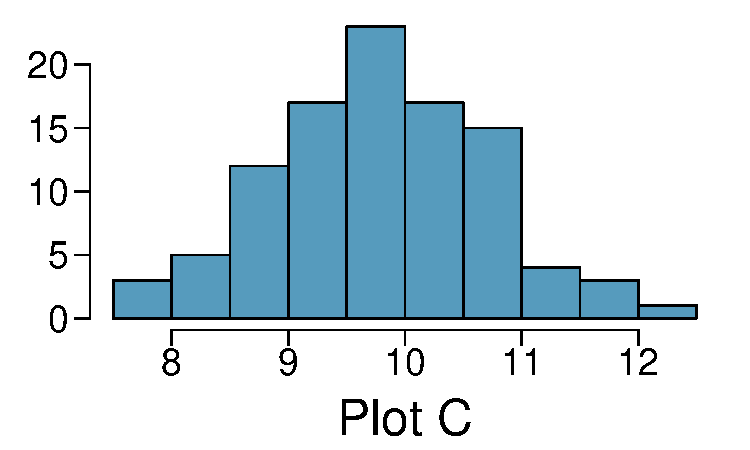
\includegraphics[width=0.32\textwidth]{4-4_clt/cltSimRS_n49.pdf}

\end{frame}

%%%%%%%%%%%%%%%%%%%%%%%%%%%%%%%%%%%%


%%%%%%%%%%%%%%%%%%%%%%%%%%%%%%%%%%%%

\section{4.5. Inferência para outras estimativas}

%%%%%%%%%%%%%%%%%%%%%%%%%%%%%%%%%%%%

\begin{frame}
\frametitle{Inferência para outras estimativas}

\begin{itemize}
\justifying
\item A média amostral não é a única estimativa pontual para a qual a distribuição amostral é quase normal. Por exemplo, a distribuição amostral das proporções da amostra também é quase normal quando $ n $ é suficientemente grande.
\justifying
\item Um pressuposto importante sobre as estimativas pontuais é que elas são \hl {imparciais}, ou seja, a distribuição amostral da estimativa é centrada no parâmetro populacional verdadeiro que se está estimando.

\begin{itemize}
\justifying
\item Ou seja, uma estimativa imparcial não sobrestima ou subestima o parâmetro. Em vez disso, ele tende a fornecer uma estimativa "boa".
\justifying
\item A média da amostra é um exemplo de uma estimativa pontual imparcial, assim como cada um dos exemplos que introduzimos nesta seção.
\end{itemize}
\end{itemize}
\end{frame}
%%%%%%%%%%%%%%%%%%%%%%%%%%%%%%%%%%%%

\begin{frame}
\frametitle{Inferência para outras estimativas}

\begin{itemize}
\justifying
\item Algumas estimativas pontuais seguem distribuições diferentes da distribuição normal, e alguns cenários requerem técnicas estatísticas que ainda não foram abordadas - discutiremos estas no final desta seção.

\end{itemize}

\end{frame}

%%%%%%%%%%%%%%%%%%%%%%%%%%%%%%%%%%%%

\subsection{Intervalos de confiança para estimativas pontuais quase normais}

%%%%%%%%%%%%%%%%%%%%%%%%%%%%%%%%%%%%

\begin{frame}
\frametitle{Intervalos de confiança para estimativas pontuais quase normais}
\justifying
Um intervalo de confiança baseado em uma estimativa pontual imparcial e quase normal é

\[ estimativa~pontual~ z^\star~ SE  \]
\justifying
onde $z^\star$ é selecionado para corresponder ao nível de confiança e SE representa o erro padrão.

$\:$ \\
\justifying
Lembre-se que o valor $z^\star~ SE$ é chamado de \hl{margem de erro}.

\end{frame}

%%%%%%%%%%%%%%%%%%%%%%%%%%%%%%%%%%%

\begin{frame}
\frametitle{Prática}

\justifying
\pq{Um dos primeiros exemplos de assimetria comportamental é uma preferência em humanos por virar a cabeça para a direita, e não para a esquerda, durante as últimas semanas de gestação e nos primeiros 6 meses após o nascimento. Acredita-se que isso influencie o desenvolvimento subsequente das preferências perceptivas e motoras. Um estudo de 124 casais descobriu que 64,5\% viravam a cabeça para a direita quando se beijavam. O erro padrão associado a essa estimativa é de aproximadamente 4\%. Qual das opções abaixo é \emph{falsa}?}

\end{frame}
%%%%%%%%%%%%%%%%%%%%%%%%%%%%%%%%%%%

\begin{frame}

\frametitle{Prática}

\begin{enumerate}[(a)]
\justifying
\solnMult{O intervalo de confiança de 95\% para a porcentagem de casais que durante o beijo viram suas cabeças para a direita é aproximadamente $64.5\% \pm 4\%$.}
\justifying
\item Um tamanho de amostra maior produziria um erro padrão menor.
\justifying
\item A margem de erro para um intervalo de confiança de 95\% para a porcentagem de casais que durante o beijo viram a cabeça para a direita é de aproximadamente 8\%.
\justifying
\item O intervalo de confiança de 99,7\% para a porcentagem de casais que durante o beijo viram a cabeça para a direita é aproximadamente $64.5\% \pm 12\%$.
\end{enumerate}


\vfill
\justifying
\ct{G\"{u}nt\"{u}rk\"{u}n, O. (2003) Adult persistence of head-turning asymmetry. \textit{Nature}. Vol 421.}

\end{frame}

%%%%%%%%%%%%%%%%%%%%%%%%%%%%%%%%%%%%

\subsection{Teste de hipóteses para estimativas pontuais quase normais}

%%%%%%%%%%%%%%%%%%%%%%%%%%%%%%%%%%%

\begin{frame}
\frametitle{Teste de hipóteses para estimativas pontuais quase normais}
\justifying
\dq{A terceira Pesquisa Nacional de Exame de Saúde e Nutrição coletou dados do percentual de gordura corporal (BF \%) e gênero de 13.601 indivíduos com idades entre 20 e 80 anos. A média de BF\% para os 6.580 homens da amostra foi de 23,9 e esse valor foi de 35,0 para as 7.021 mulheres. O erro padrão para a diferença entre a média do BF\%s de homens e mulheres foi de 0,114. Esses dados fornecem evidências convincentes de que homens e mulheres têm médias diferentes de BF\%s. Você pode assumir que a distribuição da estimativa pontual é quase normal.}

\end{frame}
%%%%%%%%%%%%%%%%%%%%%%%%%%%%%%%%%%%
\begin{frame}
\frametitle{Teste de hipóteses para estimativas pontuais quase normais}

\begin{enumerate}
\justifying
\item[1.] Definir hipóteses
\justifying
\item[2.] Calcular estimativa pontual
\justifying
\item[3.] Verificar condições
\justifying
\item[4.] Desenhar distribuição amostral, sombrear o p-valor
\justifying
\item[5.] Calcular estatísticas de teste e o p-valor, tomar uma decisão
\end{enumerate}

\end{frame}

%%%%%%%%%%%%%%%%%%%%%%%%%%%%%%%%%%%

\begin{frame}
\frametitle{Teste de hipóteses para estimativas pontuais quase normais}

\begin{enumerate}
\justifying
\item[1.] A hipótese nula é que homens e mulheres têm a mesma média de BF\% e a alternativa é que esses valores são diferentes.
\[ H_0: \mu_{homem} = \mu_{mulher} \qquad H_A: \mu_{homem} \ne \mu_{mulher} \]

\pause
\justifying
\item [2.]O parâmetro de interesse é a diferença média nas médias populacionais de BF\%s para homens e mulheres, e a estimativa pontual para esse parâmetro é a diferença entre as duas médias amostrais:
\[ \bar{x}_{homem} - \bar{x}_{mulher} = 23.9 - 35.0 = -11.1 \]

\pause
\justifying
\item[3.] Estamos assumindo que a distribuição da estimativa pontual é quase normal (discutiremos detalhes para verificar essa condição no próximo capítulo, no entanto, dado o grande tamanho de amostra, a suposição de normalidade aprece adequada).

\end{enumerate}


\end{frame}

%%%%%%%%%%%%%%%%%%%%%%%%%%%%%%%%%%%

\begin{frame}
\frametitle{Teste de hipóteses para estimativas pontuais quase normais}

\begin{enumerate}
\justifying
\item[4.] A distribuição amostral será centralizada na hipótese nula ($\mu_{homem} - \mu_{mulher} = 0$), e o p-valor é a área além da diferença observada nas médias amostrais em ambas as caudas (menor que -11,1 e maior que 11,1).

\begin{center}
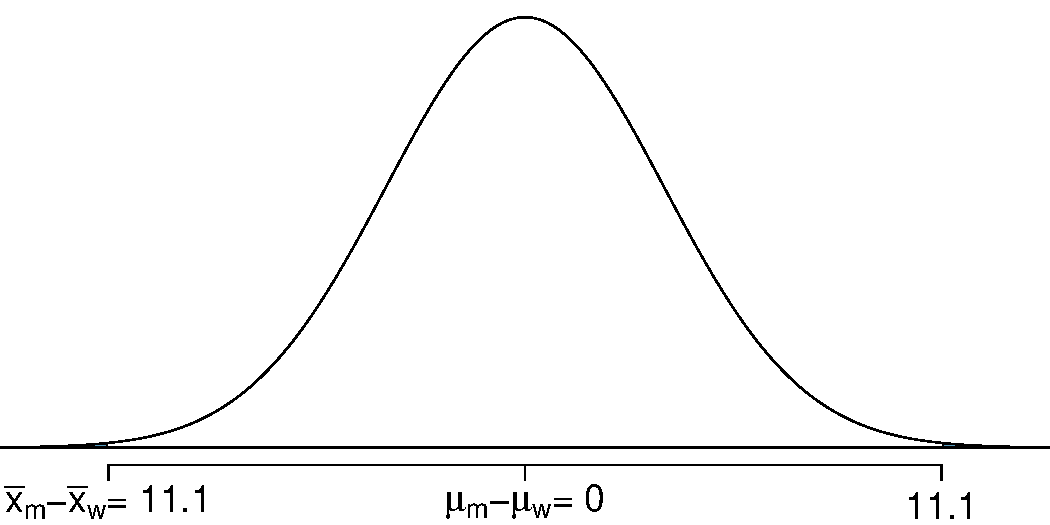
\includegraphics[width=0.75\textwidth]{4-5_inf_other_est/bf.pdf}
\end{center}


\end{enumerate}

\end{frame}

%%%%%%%%%%%%%%%%%%%%%%%%%%%%%%%%%%%

\begin{frame}
\frametitle{Teste de hipóteses para estimativas pontuais quase normais}
\begin{enumerate}
\justifying
\item[5.] A estatística de teste é calculada como a diferença entre a estimativa pontual e o valor nulo (-11.1 - 0 = -11.1), escalada pelo erro padrão.

\[ Z = \frac{11.1 - 0}{0.114} = 97.36 \]
\justifying
O valor de Z é enorme! E, portanto, o p-valor será pequeno, permitindo-nos rejeitar $H_0$ em favor de $H_A$.

\pause

$\:$ \\
\justifying
Esses dados fornecem evidências convincentes de que a média de BF\% de homens e mulheres é diferente.

\end{enumerate}

\end{frame}

%%%%%%%%%%%%%%%%%%%%%%%%%%%%%%%%%%%

\subsection{Estimativas pontuais não normais}

%%%%%%%%%%%%%%%%%%%%%%%%%%%%%%%%%%%

\begin{frame}
\frametitle{Estimativas pontuais não normais}

\begin{itemize}
\justifying
\item Podemos aplicar as ideias de intervalos de confiança e testes de hipóteses aos casos em que a estimativa pontual ou a estatística de teste não é necessariamente normal. Existem muitas razões pelas quais tal situação pode surgir:
\begin{itemize}
\justifying
\item o tamanho da amostra é muito pequeno para que a aproximação normal seja válida;
\justifying
\item a estimativa de erro padrão pode ser ruim; ou
\justifying
\item a estimativa pontual tende para alguma distribuição que não é a distribuição normal.
\end{itemize}
\justifying
\item Para cada caso em que a aproximação normal não é válida, nossa primeira tarefa é sempre entender e caracterizar a distribuição amostral da estimativa pontual ou estatística de teste. Em seguida, podemos aplicar as estruturas gerais para intervalos de confiança e testes de hipóteses a essas distribuições alternativas.

\end{itemize}

\end{frame}

%%%%%%%%%%%%%%%%%%%%%%%%%%%%%%%%%%%

\subsection{Quando recuar}

%%%%%%%%%%%%%%%%%%%%%%%%%%%%%%%%%%%

\begin{frame}
\frametitle{Quando recuar}

\begin{itemize}
\justifying
\item As ferramentas estatísticas dependem das duas condições principais a seguir:
\begin{itemize}
\justifying
\item \hlGr{Independência} Uma amostra aleatória de menos de 10\% da população assegura a independência das observações. Em experimentos, isso é garantido por amostragem aleatória. Se a independência falhar, técnicas avançadas devem ser usadas e, em alguns casos, a inferência pode não ser possível.
\justifying
\item \hlGr{Tamanho e viés da amostra} Por exemplo, se o tamanho da amostra for muito pequeno, o viés muito forte ou valores extremos estiverem presentes, o modelo normal da média da amostra falhará.
\end{itemize}
\end{itemize}

\end{frame}
%%%%%%%%%%%%%%%%%%%%%%%%%%%%%%%%%%%

\begin{frame}
\frametitle{Quando recuar}

\begin{itemize}
\justifying
\item Sempre que as condições não forem satisfeitas para uma técnica estatística:
\begin{enumerate}
\justifying
\item Aprenda novos métodos apropriados para os dados. 
\justifying
\item Consulte um estatístico.
\justifying
\item \sout{Ignorar o fracasso das condições.} Esta última opção efetivamente invalida qualquer análise e pode desacreditar descobertas novas e interessantes.
\end{enumerate}

\end{itemize}

\end{frame}

%%%%%%%%%%%%%%%%%%%%%%%%%%%%%%%%%%%

\subsection{Significância estatística versus significado prático}

%%%%%%%%%%%%%%%%%%%%%%%%%%%%%%%%%%%

\begin{frame}
\frametitle{Prática}
\justifying
\pq{Todo o resto é igual, o p-valor será menor se $n = 100$ ou $n = 10,000$?}

\begin{enumerate}[(a)]
\item $n = 100$
\solnMult{$n = 10,000$}
\end{enumerate}

\soln{\pause \pause
Suponha $\bar{x} = 50$, $s = 2$, $H_0: \mu = 49.5$, e $H_A: \mu > 49.5$.\\
\pause
\begin{eqnarray*}
Z_{n = 100} &=& \frac{50 - 49.5}{\frac{2}{\sqrt{100}}} \pause = \frac{50 - 49.5}{\frac{2}{10}} = \frac{0.5}{0.2} = 2.5,~~~\text{p-valor} = 0.0062 \\
\pause
Z_{n = 10000} &=& \frac{50 - 49.5}{\frac{2}{\sqrt{10000}}} \pause = \frac{50 - 49.5}{\frac{2}{100}} = \frac{0.5}{0.02} = 25,~~~\text{p-valor} \approx 0
\end{eqnarray*}
\pause
\begin{center}
Como $ n $ aumenta - $SE$ $\downarrow$, $Z$ $\uparrow$, p-valor $\downarrow$
\end{center}
}

\end{frame}

%%%%%%%%%%%%%%%%%%%%%%%%%%%%%%%%%%%%

\begin{frame}
\frametitle{Prática}
\justifying
\dq{Teste a hipótese $H_0: \mu = 10$ vs. $H_A: \mu > 10$ para as 8 amostras seguintes. Assuma $\sigma = 2$.}

\begin{center}
\renewcommand\arraystretch{1.5}
\begin{tabular}{l | c | c | c | c}
\hline
$\bar{x}$		& $10.05$ 	& $10.1$ 		& $10.2$  		 \\ 
\hline
\hline
\orange{$n = 30$}  
	& \soln{\only<1>{\textcolor{white}{$p-valor = 0.45$}}		\only<2->{$p-valor = 0.45$}}	
	& \soln{\only<1-3>{\textcolor{white}{$p-valor = 0.39$}}		\only<4->{$p-valor = 0.39$}} 		
	& \soln{\only<1-5>{\textcolor{white}{$p-valor = 0.29$}}		\only<6->{$p-valor = 0.29$}} \\
\hline
\hline
\orange{$n = 5000$} 
	& \soln{\only<1-2>{\textcolor{white}{$p-valor = 0.39$}}		\only<3->{$p-valor = 0.04$}}	
	& \soln{\only<1-4>{\textcolor{white}{$p-valor = 0.0002$}}		\only<5->{$p-valor = 0.0002$}}	
	& \soln{\only<1-6>{\textcolor{white}{$p-valor \approx 0$}}	\only<7->{$p-valor \approx 0$}}	 \\
\hline
\end{tabular}
\end{center}

\pause
\justifying
\soln{\only<8->{Quando $n$ é grande, mesmo pequenos desvios da hipótese nula (tamanhos de efeito pequenos), que podem ser considerados praticamente insignificantes, podem produzir resultados estatisticamente significativos.}}

\end{frame}

%%%%%%%%%%%%%%%%%%%%%%%%%%%%%%%%%%%%

\begin{frame}
\frametitle{Significado estatístico vs. prático}

\begin{itemize}
\justifying
\item Diferenças reais entre a estimativa pontual e a hipótese nula são mais fáceis de detectar com amostras maiores.
\justifying
\item No entanto, amostras muito grandes resultarão em significância estatística mesmo para pequenas diferenças entre a média da amostra e a hipótese nula (\hl{efeito de tamanho}), mesmo quando a diferença não for praticamente significativa.
\justifying
\item Isso é especialmente importante para a pesquisa: se conduzirmos um estudo, queremos nos concentrar em encontrar resultados significativos (queremos que as diferenças observadas sejam reais, mas também grandes o bastante para serem importantes).
\justifying
\item O papel de um estatístico não é apenas na análise de dados, mas também no planejamento e projeto de um estudo.
\end{itemize}

\end{frame}
%%%%%%%%%%%%%%%%%%%%%%%%%%%%%%%%%%%%
\begin{frame}
\frametitle{Significado estatístico vs. prático}

\justifying
\begin{center}{\footnotesize
\textit{``Chamar o estatístico após o término do experimento pode não ser mais do que pedir que ele faça um exame post-mortem: ele pode ser capaz de lhe dizer porque o experimento morreu.''} -- R.A. Fisher
}\end{center}

\end{frame}

%%%%%%%%%%%%%%%%%%%%%%%%%%%%%%%%%%%%




%%%%%%%%%%%%%%%%%%%%%%%%%%%%%%%%%%%%
% End document
%%%%%%%%%%%%%%%%%%%%%%%%%%%%%%%%%%%%

\end{document}